\documentclass{thesis}[2019/04/30]

% Dolgozat metaadatai
\title{Loreplotter alkalmazás fejlesztése}
\date{2019}

% Szerző metaadatai
\author{Győri Sándor}
\degree{programtervező informatikus BSc}

% Témavezető(k) metaadatai
\supervisor{Abonyi-Tóth Andor}
\affiliation{egyetemi adjunktus}
%\extsupervisor{Külső Kornél}
%\extaffiliation{informatikai igazgató}

% Egyetem metaadatai
\university{Eötvös Loránd Tudományegyetem}
\faculty{Informatikai Kar}
\department{Programozáselmélet és Szoftvertechnológiai}
\departmentSecondLine{Tanszék}
\city{Budapest}
\logo{elte_cimer_szines}

% Irodalomjegyzék hozzáadása
\addbibresource{thesis.bib}

% A dolgozat
\begin{document}

% Nyelv kiválasztása
\documentlang{magyar}
%\documentlang{english}

% Teendők listája - final dokumentumban nincs
% \listoftodos[\todolabel]

% Lábjegyzet folytonos számozása fejezetek között
\counterwithout{footnote}{chapter}

% Címlap - kötelező
\maketitle

% Tartalomjegyzék - kötelező
\tableofcontents
\cleardoublepage

% Tartalom
\chapter{Bevezetés}
\label{ch:intro}

Az író eszközei az utóbbi évtizedekben ‒ habár más formában ‒ ugyanúgy az írott szöveg egy-egy formájában testesültek meg. A történetek számtalan karakterének egyéni céljait, érzéseit, állapotát követni fejben lehetetlen. A karakterlapok pedig néha nem árulnak el minden információt, összedőlnek saját súlyuk alatt.

Ez az alkalmazás nem hivatott lecserélni a meglévő módszereket, hanem egy új eszközként lépne az iró repertoárjába. Olyan, egyébként írásban nehezen követhető, információt szolgáltat vizuálisan mellyel további segítséget tud nyújtani a történet konzisztenciájának megőrzésére, az ellentmondások elkerülésére. Ilyen például a karakterek térbeli pozíciójának és sebességének a nyílvántartása, mellyel pontosan meghatározható mennyi időnek kell elkelnie, hogy két, távol lévő karakter találkozhasson. Hordozott információik bármikor megváltozhatnak, és ezek befolyásolhatják a jövőbeli interakcióikat. Ezeket pedig habár egy papírlapra is fel lehetne vinni, az kevés teret ad a változtatásra. Egy, a történet elején lévő pillanat megváltozatása, kihathat mindenre ami utána jön. Valamint vizuális visszajelzést is nyújt azzal, hogy lejátszhatóvá teszi a felvitt adatokat. Webalkalmazás lévén pedig könnyen hozzáférhető bárki számára.

\cleardoublepage

% !TeX root = ../thesis.tex
\chapter{Felhasználói dokumentáció}
\label{ch:user}

Az alkalmazás sem telepítést sem regisztrációt nem igényel, teljes egészében böngészőből használható. Minden alkalmazáson belüli tevékenység egy projekthez köthető melyeket a felhasználó kedve szerint hozhat létre, törölhet, módosíthat. Egyszerre több projektet is vezethetünk, a váltás közöttük azonnali.

\section{A Projekt}

Minden projekt\cref{fig:basic-project-structure} három fő elemből áll, ezek a név, a világ és később a szereplők. Új projekt létrehozásakor a projekt nevét és a világának adatait szükséges megadni.

\begin{figure}[h!]
	\centering
	\begin{forest}
		forked edges,
		for tree={edge+={-Latex}},
		[Projekt
			[Név]
			[Világ [Név] [Méret]]
			[Szereplők [\dots]]
		]
	\end{forest}
	\caption{
		Projektstruktúra}
	\label{fig:basic-project-structure}
\end{figure}

\begin{figure}[h!]
	\centering
	\includegraphics[width=0.50\textwidth,scale=1]{create-project-button}
	\caption{
		Új projektet létrehozni a jobb felső sarokban található menü legfelső elemével tehetjük meg}
	\label{fig:create-project-button}
\end{figure}

Új projekt létrehozásakor a projekt készítő dialógust kapjuk melyen lehetőséget kapunk a projektünknek a nevét, a világ nevét és méretét megadni, utóbbi alatt a bolygó sugarát értjük kilóméterben megadva. Valamint egy tetszőleges fekete-fehér magasságtérképet is megadhatunk amivel inicializálhatjuk a bolygó felületét. A vízmagasság alapértelmezetten 40\%-os szürkeségnél van. A 'Create' gombra kattintva azonnal megnyílik az elkészített projekt.

\begin{figure}[h!]
	\centering
	\includegraphics[width=0.80\textwidth,scale=1]{create-project-form}
	\caption{
		Új projekt dialógus}
	\label{fig:create-project-form}
\end{figure}


\begin{table}[H]
	\centering
	\begin{tabular}{ | m{0.25\textwidth} | m{0.10\textwidth} | m{0.55\textwidth} | }
		\hline
		\textbf{Mező} & \textbf{Típus} & \textbf{Leírás} \\
		\hline \hline
		\emph{Név} & Szöveg & Kötelező. Egyedi. A projekt azonosítója. \\
		\hline
		\emph{Bolygó név} & Szöveg & Kötelező. Alapértelmezett értéke: "Earth" \\
		\hline
		\emph{Bolygó méret} & Szám & Kötelező. Alapértelmezett értéke: "6371". (A föld sugara kilóméterben). Minimum 500.  \\
		\hline
		\emph{Magasságtérkép} & Kép & Opcionális. Egy tetszőleges kezdeti magasságtérkép  \\
		\hline
	\end{tabular}
	\caption{Új projekt sablon}
	\label{tab:create-project-form}
\end{table}

Meglévő projektet szerkeszteni a menü gomb mellett a projekt nevére kattintva lehet. Itt lehetőség van megváltoztatni a készítéskor megadott adatokat, új textúrát felölteni, esetleg betölteni az alapértelmezett föld textúrát. Szerkesztéskor bejön a képbe egy új megszorítás. Mivel a szereplőinknek meg kell tudniuk tenni bármely két esemény között a távot a saját sebességüknek megfelelően így itt limitálva van a bolygó maximális mérete aszerint, hogy ez a feltétel még ne sérüljön.

\begin{figure}[h!]
	\centering
	\includegraphics[width=1\textwidth,scale=1]{edit-project-form}
	\caption{
		Projekt szerkesztése dialógus}
	\label{fig:create-project-form}
\end{figure}

\pagebreak

\section{A Kezelőfelület} \label{section:ui}

\begin{figure}[h!]
	\centering
	\includegraphics[width=1.0\textwidth,scale=1]{full-screenshot-open-sidebar}
	\caption{
		A kezelőfelület}
	\label{fig:full-screenshot-open-sidebar}
\end{figure}

A kezelőfelület az alábbi elemeket tartalmazza:

\begin{itemize}
	\item Bal oldalt a szereplőtár\cref{section:ui-actor-tool} amivel készíteni és válogatni tudunk a szereplőink között.
	\item Alul az idővonal\cref{section:ui-timeline} látható ahol a jelenlegi időt és a szereplők eseményeit tudjuk megváltoztatni.
\end{itemize}

\subsection{A Szereplőtár} \label{section:ui-actor-tool}

A szereplőtár legfelső elemével lehet újabb szereplőket hozzáadni a színtérhez. A gombot fogd-és-vidd módon lehet a bolygó bármely pontjára ráhúzni, ami majd a karakter kiindulási pontja lesz. Ez akármikor megváltoztatható, amíg egyedül van pedig korlátok nélkül.

Ez alatt az elkészített karakterek listája van, mellette az összes karakter számával. Egy karakter itt az alábbi információt tartalmazza:

\begin{itemize}
	\item Név (Akkumulált a jelenlegi időpillanatra)
	\item Szín (Akkumulált a jelenlegi időpillanatra)
	\item Összes esemény száma
\end{itemize}

A szereplőtár legalján van a 'Debug mód' gomb is amivel bekapcsolhatunk a színtéren azon vektorok vizualizációját amik az események távolságainak metszetét számolják és tartják az éppen manipulált szereplőt a metszetben.

\begin{figure}[h!]
	\centering
	\includegraphics[width=0.5\textwidth,scale=1]{debug}
	\caption{A debug toolt bekapcsolva láthatjuk akció közben ezeket a számításhoz használt vektorokat.}
	\label{fig:debug}
\end{figure}
\begin{figure}[h!]
	\centering
	\includegraphics[width=0.5\textwidth,scale=1]{debug2}
	\caption{Egy másik szögből egy metszéspont eset. A fehér vektorok az egér pozíciója felé mutatnak.}
	\label{fig:debug2}
\end{figure}




\pagebreak
\subsection{Az Idővonal} \label{section:ui-timeline}

A idővonalat elsősorban három elemre tudjuk bontani:

\subsubsection{A Kurzor}

A vonalzón helyezkedik el. Mindig a jelenlegi időpontra mutat, melyet a kurzoron, fogd-és-vidd módszerrel megváltoztathatunk. Egy fölötte megjelenő buborék a pontos időt mutatja másodperc pontossággal. Ez egyben szerkeszthető is ha egy konkrét időpontra akarunk ugrani. Ha átszerkesztettük az időpontot a kurzoron akkor az 'Enter' billentyűvel a megadott időpontra ugrik. Ha megváltozik az idő akkor az azonnal bekerül értékként ide így lejátszás közben ez nem szerkeszthető.

\paragraph{A Vonalzó}

Beosztásai napokban értendőek, a kisebb fogai pedig óráknak. A vonalzót fogd és vidd módon tudjuk az időben előre vagy hátra eltolni. Az egérgörgővel pedig az aktív idősávot tudjuk kibővíteni, szűkíteni. A legközelebbi megengedett nagyítás 2 napot foglal magában.

\paragraph{A Karakter Sávok}

Minden karakter saját sávval rendelkezik. Bal oldalt a sávhoz tartozó karakter akkumulált nevét lehet látni. A sávon belül pedig a blokkját ami eseményekre van felosztva.

Egy blokk az alábbi interakciós lehetőségeket nyújtja:
\begin{enumerate}
	\item Egy eseményre kattintva a kurzor arra az időpontra ugrik és az esemény kiválasztásra kerül. Kiválasztás után lehetőség van kitörölni az adott eseményt egy megerősítést követően. Emellett kiválasztásra kerül a hozzá tartozó szereplő is a színtéren. Eseményt törölni csak akkor lehet ha törlést követően az előző esemény helyéről még elérhető a következő.
	\item Egy esemény fogd-és-vidd módon áthelyezhetünk bárhova az idővonalon. A művelet érvénytelen ha az környező események megengedett sebességei és távolsága alapján a szereplő már nem tudná teljesíteni az adott utat. Ha ez sérül akkor a művelet érvénytelen és az esemény visszaugrik eredeti pozíciójára. Figyeljünk oda, hogy ha a jövőben egy esemény függ ettől, és egy annál későbbi időpontra helyezzük, akkor ez a függőség sérül. Ez viszont már nincs ellenőrizve.
	\item A blokk egészét is mozgathatjuk fogd és vidd módon, ezzel az összes esemény párhuzamosan fog elmozdulni. Figyeljünk oda, hogy ha egy másik szereplő egy vagy több eseménye függ a mozgatott szereplő eseményeitől, akkor ezek a függőségek sérülhetnek. Ez nincs ellenőrizve.
	\item Az egeret a karakter sávja felett tartva a színtéren a hozzá tartozó objektum körül egy körvonal jelenik meg a gyors azonosításért. Ez akkor is látszik ha a szereplő a bolygó másik oldalán van.
\end{enumerate}

Az idővonalon egyszerre 4 sáv fér el. A többi sávot görgetéssel, függőleges pásztázással, vagy a görgősávval érjük el.

\subsection{A Színtér} \label{section:ui-scene}

A kezelőfelület közepén helyezkedik el a 3D színtér és az azt közvetlen kezelő eszközök. A színtér fő eleme a bolygó és rajta a szereplők. A bolygó mozgatás módban a felületét pásztázva forgatható, az egérgörgővel pedig közelíthető/távolítható.

A bolygó felületén lévő szereplők helyét, a szereplőt reprezentáló színes gömb fogd-és-vidd módon történő áthelyezésével lehet megtenni. Ennek a viselkedése nagyban függ a jelenlegi időtől és a szereplő azon eseményeitől mely a jelenlegi időponton, vagy a körül helyezkednek el. Minden szereplő rendelkezik egy maximum elérhető sebességgel. Hogy ez be legyen tartva, egy szereplő áthelyezésekor, csak olyan távolságba engedett az áthelyezés, amivel még el lehet érni az előző és a következő esemény helyét. Egy esemény helye áthelyezhető ha áthelyezéskor az az esemény ideje van kiválasztva, egyéb esetekben új esemény jön létre.


\subsubsection{Eszközök} \label{section:ui-utilities}

A színtér 3 sarkában 3 eszköztár látható.

\subsubsection{Az interakciós eszköztár}

\begin{figure}[h!]
	\centering
	\includegraphics[width=0.60\textwidth,scale=1]{tool-interaction}
	\caption{Interakciós eszköztár, a színtér bal felső részén.}
	\label{fig:tool-interaction}
\end{figure}

A ceruza ikonnal ellátott gombbal rajzolás módba válthatunk, a mellette lévő két csúszka pedig az ecset paraméterei: magasság és méret. A bolygó felületét pászázva azt megváltoztathatjuk. Alacsony magassággal tengereket is rajzolhatunk. A bolygón kívül pásztázva ugyanúgy forgathatjuk mintha mozgatás módban lennénk.

A tengely ikonnal ellátott gombbal az alap, színtér mozgatáshoz szükséges módba térhetünk vissza. A mellette lévő csúszka a szereplőket reprezentáló gömbök méretét állítja. A gömbök mérete ettől, és a közelítés mértékétől is függ.

\subsubsection{Az fény eszköztár}

\begin{figure}[h!]
	\centering
	\includegraphics[width=0.20\textwidth,scale=1]{tool-light-manual-light}
	\caption{A fény eszköztár manuális módban, világosra állítva. A színtér bal alsó részén.}
	\label{fig:tool-light-manual-light}
\end{figure}

A kör alakú gombbal manuális és automata módok között válthatunk. A jobb oldali gomb csak manuális módban látszik. Ezzel tudunk váltani az állandó világos és a sötét mód között.

\paragraph{Világos mód}

Világos módban a kezelőfelület teljes egésze fehérre vált, ahogy színtér háttere is. A színtérben a nap eltűnik és a bolygó egésze megvilágításra kerül.

\paragraph{Sötét mód}

Sötét módban a kezelőfelület teljes egésze sötétre vált, ahogy a színtér háttere is. A színtérben a nap csak ebben a módban van jelen, és a bolygót érő legerősebb fényforrássá válik. Ebben a módban is változhat a megvilágítás a sebességnek megfelelően. \ref{fig:tool-time}

\paragraph{Automata mód}

Automata módban alapértelmezetten a sötét mód aktív de túl közeli zoomnál, vagy akkor ha az idő túl gyorsan telik automatikusan a világos mód kapcsol be.

\subsubsection{Az idő eszköztár}

\begin{figure}[h!]
	\centering
	\includegraphics[width=0.40\textwidth,scale=1]{tool-time}
	\caption{Az idő eszköztár, a színtér jobb alsó részén}
	\label{fig:tool-time}
\end{figure}

Az idő eszköztár fő eleme a lejátszás gomb. Erre kattintva a csúszkával vagy a gombokkal beállított sebességgel megkezdődik a lejátszás. A sebesség egysége egy percet jelent minden valódi másodpercre. A lejátszás megkezdésével a színtér szereplői az eseményeik pozíciói között fognak mozogni.

Az alábbi billentyűkkel is vezérelhető a lejátszás:

\begin{table}[H]
	\centering
	\begin{tabular}{ | m{0.15\textwidth} | m{0.55\textwidth} | }
		\hline
		\textbf{Billentyű} & \textbf{Hatás}\\
		\hline \hline
		\emph{Szóköz} & A lejátszás megkezdése, szünetelése. \\
		\hline
		\emph{Számok 0-9} & A kettő adott hatványával való lejátszás. \\
		\hline
		\emph{Jobbra nyíl} & A lejátszás irányát pozitívra állítja.  \\
		\hline
		\emph{Balra nyíl} & A lejátszás irányát negatívra állítja.  \\
		\hline
		\emph{Felfele nyíl} & A lejátszást gyorsítja 60 egységgel. \\
		\hline
		\emph{Lefele nyíl} & A lejátszást lassítja 60 egységgel.  \\
		\hline
	\end{tabular}
	\caption{Idő vezérlése gombokkal}
	\label{tab:tool-time-control-keys}
\end{table}

\subsection{A Szereplők} \label{section:ui-actors}

A színtér szereplői kattintással, egy eseményét kiválasztva vagy a bal oldali menüből is kiválaszthatóak. Kiválasztást követően egy kis ablak jelenik meg a szereplő színtérbeli pozíciójánál mutatva az összes akkumulált adatát, és hogy melyik eseménynél lett utoljára módosítva. Utóbbi gombra kattintva a kurzor egyből arra az időre ugrik. A tetején van két speciális gomb amikkel a legkorábbi és a legkésőbbi eseményhez ugorhatunk. Ugrás közben az időablak követi a kurzort így az sose megy ki a képernyőről. Hasznos ha az időablak nagyon messzire elment.

\begin{figure}[h!]
	\centering
	\includegraphics[width=0.40\textwidth,scale=1]{actor-popup}
	\caption{Az szereplő ablaka a jelenlegi adataival}
	\label{fig:actor-popup}
\end{figure}

A szerkesztés gombra kattintva pedig az adott időpillanat, adott helyzetén szerkeszthetjük a szereplő adatait. Minden változtatás a fent megjelenő időtől lesz érvényes. Egy ilyen változtatás nem befolyásolja a karakter pozícióját, mentéskor a megadott dátum alapján -- ugyanúgy ahogy a lejátszás teszi -- kiszámolja, hogy hol tartózkodna akkor a szereplő és azzal a helyzettel menti el az eseményt.

\begin{table}[H]
	\centering
	\begin{tabular}{ | m{0.25\textwidth} | m{0.10\textwidth} | m{0.55\textwidth} | }
		\hline
		\textbf{Mező} & \textbf{Típus} & \textbf{Leírás} \\
		\hline \hline
		\emph{Dátum} & Szöveg & Megváltoztatható a szerkesztés dátuma. \\
		\hline
		\emph{Idő} & Szöveg & Megváltoztatható a szerkesztés időpontja. \\
		\hline
		\emph{Név} & Szöveg & A szereplő neve.  \\
		\hline
		\emph{Maximális sebesség} & Szám & A szereplő sebessége kilóméter per órában. \\
		\hline
		\emph{Szín} & Szín & A szereplő színe. \ref{fig:actor-edit-dialog-color}  \\
		\hline
	\end{tabular}
	\caption{Szereplő alap adatai}
	\label{tab:create-project-form}
\end{table}

\begin{figure}[h!]
	\centering
	\includegraphics[width=0.70\textwidth,scale=1]{actor-edit-dialog}
	\caption{Az szereplő szerkesztés abalaka}
	\label{fig:actor-edit-dialog}
\end{figure}

A szereplőnek lehetnek már meglévő, akkumulált tulajdonságai is mikor az ablakot megnyitjuk. Ezeket értékét megváltozathatjuk, de kitörölni itt nem tudjuk, ugyanis nem itt születtek. De "elfelejthetjük" őket aminek hatására az adott időpillanat után már nem lesz jelen a tulajdonság.

Lehetőség van új tulajdonságok felvitelére is, itt jelennek meg az adott eseményen született tulajdonságok is. Ezek törölhetőek mert nem akkumulált adatok.

\begin{figure}[h!]
	\centering
	\includegraphics[width=0.30\textwidth,scale=1]{actor-edit-dialog-color}
	\caption{Az szereplő színének megváltoztatása}
	\label{fig:actor-edit-dialog-color}
\end{figure}


\subsection{Az import/export eszköz} \label{section:ui-import-export}

Lehetőség van az adatbázist szöveges formában kimenteni, beolvasni. Ezt a menü (\ref{fig:create-project-button}) Export gombjával nyithatjuk meg.

\begin{figure}[h!]
	\centering
	\includegraphics[width=1\textwidth,scale=1]{ui-import-export}
	\caption{Az import/export ablak}
	\label{fig:ui-import-export}
\end{figure}

Az itt megjelenő JSON \cite{JSON} reprezentálja a teljes adatbázist amit az alkalmazás használ éppen. A 'Copy to clipboard' gomb egy kattintással a vágólapra helyezi a kiexportált szöveget. Ugyanide visszamásolva, majd az import gombra nyomva, egy megerősítést követően a jelenlegi adatbázist teljesen felülírja. Figyelem, a szöveg nem tartalmazza a projektek textúráit! Ezeket külön lehet letölteni a 'Download all textures' gombbal.

\cleardoublepage

\chapter{Fejlesztői dokumentáció}
\label{ch:impl}

Az alkalmazás a könnyű megközelíthetőség miatt web alapúan kerül megvalósításra. Ennek számos előnye van. Az alkalmazás nem igényel telepítést, bármilyen számítógépről, bármikor elérhető. A már ismert webes technológiákat alkalmazhatjuk. És Progresszív Web Alkalmazás (PWA \cite{PWA}) lévén az első megnyitást leszámítva aktív internetelérés sem kell a használatához.

\section{Megoldási terv}

Az alkalmazás fő eleme a projekt amit Lore-nak nevezünk, ennek van egy azonosítója mivel dokumentum szintű objektumról van szó, egy neve és ebben tároljuk a világ adatait a nevét és méretét. Valamint ehhez a dokumentumhoz tartozik a világ textúrája is, bináris csatolmányként.

Egy projekthez tartoznak még szereplők amik szintén dokumentum szintű objektumok, saját kollekcióval. Ebben tároljuk a szereplő állapotait egy AVL fában \cite{AVL} amiben a kulcs az idő, ezzel biztosítva, hogy minden esemény idő szerint rendezett legyen, és gyorsan elérhetőek legyenek. Szükség lesz ehhez a fához néhány segédeljárásra. (Az alkalmazásban saját, gazdag API-val ellátott AVL fa implementáció használok ami NPM-en van közzétéve.)

Egy állapotdelta csak az előző állapotdeltákhoz viszonyított különbséget tartja nyilván, kivéve a pozíciót, ami minden esetben kötelező. Ezeket a deltákat a szereplők és a jelenlegi idő csöveinek összevezetésével egy aggregátoreljárás értékeli ki. Erre feliratkozva bármi azonnal hozzáférhet a legfrissebb adatokhoz ami csak egy helyen, egyszer van emiatt kiszámolva.

\subsection{Az adatmodell}
\begin{plantuml}
@startuml
skinparam monochrome true

note left of Lore: Tartozhat minden példányhoz egy\nRxDocument 'texture' azonosítóval

interface Lore {
	id: string
	name: string
	planet: Planet
}

interface Planet {
	name: string
	radius: number
}

interface Actor {
	id: string
	loreId: string
	states: Tree
}

note left of Tree: Nem perzisztálható de szérializálható
class Tree {
	root: Node
}

class Node {
	key: number
	value: ActorDelta
}

interface ActorDelta {
	position: Vec3
	name?: string
	maxSpeed?: number
	color?: string
	properties?: Array<Property>
}

interface Vec3 {
	x: number
	y: number
	z: number
}

interface Property {
	key: string
	value: string
}

Lore -- Planet
Lore --o Actor
Actor -- Tree
Tree --* Node
Node -left- ActorDelta

ActorDelta --* Property
ActorDelta -- Vec3

@enduml
\caption{Az adatmodell}
\label{fig:data-model}
\end{plantuml}

\pagebreak

\subsection{Reaktív elemek}

Az alkalmazás jelentős részében reaktív komponenseket használunk amik alapjául az RxJS \cite{RxJS} csomag szolgál. Ez azt jelenti, hogy klasszikus adattagok helyett, javarészt adatforrásokat, megfigyelhető objektumokat (Lásd Megfigyelő programtervezési minta \cite{ObserverPattern}), függvényhívások helyett pedig mellékhatásokat használunk.

Ez a minta lehetőséget ad arra, hogy bármilyen nézet a böngészőben ami felhasznál valamilyen adatot, azonnal frissüljön mikor a forrása megváltozik.

\begin{figure}[h!]
	\centering
	\begin{plantuml}
		@startuml
		skinparam monochrome true
		hide empty description
		[*] -> Observable : Új adat kerül a megfigyelhető objektumba
		Observable --> Pipes
		Pipes : A csövek formában és időben is \nmegváltoztathatják a bennük átfolyó adatot
		Pipes --> SideEffects : A transzformáció közben mellékhatásokat is definiálhatunk
		Pipes --> ObserversA
		Pipes --> ObserversB
		Pipes --> ObserversC : Majd pedig megérkeznek minden feliratkozóhoz

		SideEffects  --> [*]
		ObserversA --> [*]
		ObserversB --> [*]
		ObserversC --> [*] : És kifejtik hatásukat
		@enduml
	\end{plantuml}
	\caption{Adatfolyam a megfigyelő modellben}
	\label{fig:observer-pattern}
\end{figure}

Kétfajta adatot különböztetünk meg, perzisztens és temporális. Perzisztens adatnak minősül minden ami egy projekthez tartozik. Temporális meg az amiket az előbbi manipulálásakor használunk fel. Például projekthez tartozó adat az, hogy egy szereplőnk egy adott időpillanatban hol tartózkodik, de az nem, hogy a kurzor épp ezen az időpillanaton áll.

A perzisztens adatok a böngészők beépített IndexedDB (noSQL) adatbázisában kerülnek tárolásra, dokumentumok formájában. Az adatbázis elérésehez, és ezzel az alkalmazás reaktív modelljének alapkövének RxDB-t \cite{RxDB} használunk.

Ez a csomag lehetővé teszi, hogy adatok beszúrásakor/módosításakor/törlésekor ezek a folyamatok igéretekként (Lásd Promise \cite{Promise}) jelenjenek meg melyek teljesüléséről értesítést kapunk. Ezzel elérhetővé téve olyan lehetőségeket mint, hogy jelezni a felhasználónak, hogy egy adott elem adatainak forrása éppen mentés alatt áll, és a szerkesztését letiltani. A legfőbb előnye viszont az, hogy bármilyen adatbázis kollekciót, lekérdezést megfigyelhetünk. És amint változás történik az adatbázisban, ezek a megfigyelhető Query-k újra jeleznek, frissítve minden mást ami rájuk épül.

A temporális adatokat viszont felesleges adatbázisban tárolni csak azért, hogy reaktív módon kezelhessük őket. Lehetőség van minden ilyen adatnak egy saját forrást (Subject) biztosítani. De mi van ha két adat függ egymástól? Csöveken keresztül futtassuk őket össze, válasszuk szét majd az így keletkező csöveket használjuk ezentúl? Mi van ha erre a változtatásra később kerül sor? Mi van ha valamit elfelejtünk átállítani, hogy a direkt-forrás helyett a transzformált csövet használják? Ezek a problémák és még sok más megoldására jön képbe az NgRX \cite{NgRx} csomag és a Redux (\cite{Redux}) architektúra amit implementál.

\begin{figure}[h!]
	\centering
	\begin{plantuml}
		@startuml
		skinparam monochrome true
		hide empty description
		[*] -d-> View : Felhasználói interakció
		View -d-> Dispatcher : Akció
		Dispatcher -l-> Effects : Akció
		Effects -r-> Dispatcher : Akció
		Effects -l-> [*] : Mellékhatás

		Dispatcher --> Reducer : Akció
		CurrentState -> Reducer : Az előző állapot
		Reducer --> Store : Új állapot készül
		Store -u-> View : Értesít

		@enduml
	\end{plantuml}
	\caption{A Redux architektúra}
	\label{fig:redux-architecture}
\end{figure}

A lényeg a globális, nem módosítható (Csak cserélhető) állapot, az úgynevezett "igazság egyetlen forrása" ("Single source of truth") és az egyirányú adatfolyam (Unidirectional data-flow). Ennek hála egy átlátható, eseményeiben könnyen megjósolható programot kapunk, cserébe viszont sok kódot igényel.
Ezt egy központi Store service-ből tudjuk elérni, a könnyebb interakció miatt pedig egy Facade\cite{Facade} Service-t húzunk elé.

\section{Alkalmazás Architektúra}

Minden Angular alkalmazás modulokra van bontva. Minden modul saját Injection Scope-al rendelkezik, a felhasznált Service-ek pedig egyediek Injection Scope-onként. Mivel ez az alkalmazás csupán egy funkciót lát el megelégedhetnénk egy modullal is, de jobb felhasználói élményt érhetünk el ha az első töltést felgyorsítjuk azzal, hogy az applikációnk első töltési pontját kiürítjük, a tényleges applikációt pedig a gyökér routing pont mögé tesszük. Ez lusta módon \cite{LazyLoad} fogja betölteni a tényleges tartalommal rendelkező modult, nem blokkolva az alap modul tartalmának festését a DOM-ba. Az alap modul így taralmazhat egy egyszerű töltési animációt amit csak addig jelenítünk meg amíg a router tölti az almodult.

\begin{figure}[h!]
	\centering
	\begin{plantuml}
		@startuml
		skinparam monochrome true

		[-> AppModule: Applikáció indításakor
		activate AppModule
		AppModule -> AppModule : Első festés, LoreModule Lazy töltése

		activate  AppModule
		AppModule -> LoreModule
		deactivate AppModule

		activate LoreModule

		LoreModule ->]
		LoreModule <-]


		AppModule <- LoreModule: Kilépés
		deactivate LoreModule

		[<- AppModule: Kilépés
		deactivate AppModule

		@enduml


	\end{plantuml}
	\caption{Lusta betöltés}
	\label{fig:lazy-loading}
\end{figure}


\subsection{Komponensek}

Nézeteinket komponensekben definiáljuk, ezek az adataikat pedig kizárólag a StoreFacade-on keresztül kapják. Egyedül az Engine és a 3D színtér az ami közvetlen az adatbázissal kommunikál.

\begin{figure}[h!]
	\centering
	\begin{plantuml}
		@startuml
		skinparam monochrome true

		database IndexedDB {
			[LoreCollection]
			[ActorCollection]
		}

		database Store {
			[State]
		}

		IndexedDB -[hidden]--> LoreModule
		Store -[hidden]--> LoreModule

		IndexedDB .> (RxDB)


		package LoreModule {
			Store .> (StoreFacade)
			(RxDB) ..> (DatabaseService)
			(DatabaseService) .[hidden].> [Lore]
			(DatabaseService) <.> Engine
			Store <.. (DatabaseService)
			(StoreFacade) .> [Lore]
			(StoreFacade) .> Components
			(StoreFacade) .> Engine
			[Lore] <- Components
			node Components {

				node Control {
					[LightControl]
					[SceneControl]
					[PlayControl] --> [SpeedControl]
				}


				node Timeline {
					[Block] --> [Timeline]
					[Cursor] --> [Timeline]
				}
			}

			[Lore] <- Engine

			Engine -[hidden]-> Components

			node Engine {
				(EngineService)
				[EngineComponent]
			}


		}


		@enduml
	\end{plantuml}
	\caption{Főbb Komponensek és relációik}
	\label{fig:services-and-components}
\end{figure}


\begin{figure}[h!]
	\centering
	\begin{plantuml}
		@startuml
		skinparam monochrome true
		== Initialization ==
		[-> Database : Database Initialized
		Database --> LoreState: Load Lores
		activate LoreState
		LoreState -> LoreState: Shim each entry
		LoreState ->]: loadLoresSuccess
		deactivate LoreState
		== Loading Lores ==
		note left of LoreState : updateInitialSelectedLore
		[-> LoreState : loadLoresSuccess
		activate LoreState
		LoreState -> LoreState: Select the first one
		LoreState ->] : changeSelectedLore
		deactivate LoreState
		== On Create Lore ==
		Database --> LoreState: createLoreSuccess
		LoreState ->]: changeSelectedLore
		== On Change Selected ==
		[-> LoreState: changeSelectedLore
		LoreState ->]: changeSelectedLoreSuccess
		== Change Selected ==
		[-> ActorState: changeSelectedLoreSuccess
		activate ActorState
		Database --> ActorState: connection
		ActorState -> ActorState: Loading everything into state
		ActorState ->]: loadActorsSuccess
		deactivate ActorState
		== On Load Actors ==
		[-> ActorState: loadActorsSuccess
		activate ActorState
		ActorState -> ActorState: Deserilization of deltas
		deactivate ActorState
		@enduml
	\end{plantuml}
	\caption{Bootstrap folyamatok}
	\label{fig:global-state-bootstrap}
\end{figure}

\pagebreak

\subsection{Timeline}

Az idő az alkalmazásban epoch \cite{Epoch} formában van jelen, egy egyszerű számként, az egység a másodperc. Így könnyű egyszerű aritmetikai műveleteket végezni rajta. Minden művelet után ezt lefele kerekítjük

Az idővonalat két időpont határoz meg, az eleje és a vége. A nézet szélességét figyelembe véve ezekből ki lehet számolni a vonalzó beosztásait. A beosztásokat napokban mérjük, az albeosztásokat pedig órában.

\subsubsection{Megjelenítés}

A beosztások mennyiségét és pozícióit ki kell számolnunk. Előbbit úgy kapjuk meg ha vesszük a megjelenített időablak hosszát és leosztjuk egy nappal ($86400s$). Az egészrésze lesz a kiférő beosztások száma. Viszont az albeosztások megjelenítésére is figyelnünk kell. Ezek fixen a tőle balra álló nagy beosztástól fognak elhelyezkedni. Ahhoz, hogy az idővonal legelején is lehessenek albeosztások -- az első látszódó beosztás előtt -- el kell tolnunk balra egy egységgel az idővonalat, és a végére még kettőt hozzáadni. Egy beosztás hosszát az alábbi módon kaphatjuk meg:

\begin{tabular}{@{}ll@{}}
	& \\
	\textbf{Jel} & \textbf{Leírás} \\
	$a$ & Időablak kezdete \\
	$b$ & Időablak vége \\
	$d$ & A beosztás hossza ($86400$) \\
	$w$ & A komponens szélessége pixelben \\
	$d'$ & A beosztás szélessége pixelben \\
\end{tabular}
$$d' = \frac{w}{(b - a) / d}$$

A beosztások pozícióinak kiszámolásához, ahelyett, hogy minden beosztás helyét egyenként kiszámolnánk, csupán az első helyét számoljuk ki, a többit pedig ahhoz mérten, fix távolságban eltoljuk. Ezt azért tehetjük meg mert a beosztások egyenlő közönként vannak az idővonal egészén. Elég egyszer kiszámolni, hogy a $86400$ másodperc éppen mekkora távolságot jelent pixelben a képernyőn. Azután elég ennek a többszöröseit hozzáadni az első távolságához, minden egyes beosztásnál.

Az első távolság kiszámolásához viszont tudnunk kell, hogy melyik az a pont a kiválaszott időablakban ami egy napfordulót jelent:

$$x \in \{ y | y \in [a, a+l], y \equiv 0 \mod b\}$$

Ehhez csak hozzá kell adni a beosztás hossza és a kezdeti érték maradékát a kezdeti értékhez miután kivontuk a beosztás hosszából:

$$x = a + (d - (a \% d))$$

Az albeosztásokat már tudjuk, hogy $24 - 1$ darab fog kelleni, kezdeti pozíciójuk meg nem számít, relatív a nagy beosztáshoz vannak elhelyezve. Csak azt kell kiszámolnunk, hogy az adott albeosztás másodpercben mennyit jelent ($0, 3600, 7200 \dots $) és pixelben mért távolsággá alakítani.


A két tartomány között lineárisan váltunk. A főbeosztások esetén a kezdeti tartomány az időablak, a céltartomány pedig a $[0, w]$ ahol $w$ a komponens szélessége. Az albeosztások esetén pedig $[0, 86400]$ ból váltunk $[0, d']$ be ahol $d'$ a beosztás hossza pixelben.

\begin{tabular}{@{}ll@{}}
	& \\
	\textbf{Jel} & \textbf{Leírás} \\
	$x$ & A transzformálandó érték \\
	$a1$ & A forrás tartomány kezdete \\
	$a2$ & A forrás tartomány vége \\
	$b1$ & A cél tartomány kezdete \\
	$b2$ & A cél tartomány vége \\
\end{tabular}

$$ f(x) = b1 + ( x - a1 ) * ( b2 - b1 ) / ( a2 - a1 )$$

A beosztások így helyesen helyezkedenek el minden időablak esetében.

\subsubsection{Manipulálás}

\paragraph{Folytonos manipuláláskor} mint például mikor pásztázunk az egerünkkel, a kapott eseményben (a módosítás eseménye, Hammer Event) csak az eltolás mértékét kapjuk meg pixelben, ahhoz a pozícióhoz képest, ahol az eltolás kezdetekor az egér volt. A legtöbb ilyen esethez ezért definiálunk egy módszert amiben egy ilyen módon manipulálható adat mellé egy felülíró adattagot is definiálunk. Ez az adattag amikor nem történik esemény mindig \lstinline[columns=fixed]{undefined}.

Kiolvasni az adatpárost emiatt rövidzár kiértékeléssel egyszerű (\lstinline[columns=fixed]{override || original}). Fontos megjegyezni, hogy számok lévén, és mivel itt nem az adattag létezését vizsgáljuk hanem azt, hogy truthy e vagy sem, ha az \lstinline[columns=fixed]{override} értéke $0$ lenne, akkor ugyagyúgy az \lstinline[columns=fixed]{original} értékkel térne vissza a kifejezés. Mivel a $0$ az falsy. Így ezt csak akkor alkalmazzuk, ha tudjuk hogy ez az érték sosem lesz $0$. A másik megjegyzendő dolog, hogy miért nem egy osztályt definiálunk ennek a viselkedésnek a kezelésére. A válasz az, hogy ezek az adatok az állapot részét képezik, az állandó szérializálás és deszérializálás pedig túl sok extra komplexitást adna egy egyébként egyszerű feladathoz.

A folytonos manipuláció végén pedig az \lstinline[columns=fixed]{override} értékét beleírjuk az eredeti változóba majd kiürítjük.


A megjelenített időablakot kétféle módon manipulálhatjuk:

\begin{itemize}
	\item Eltolás (Translate)
	\item Merőleges affinitás (Scale)
\end{itemize}

\paragraph{Eltolásnál} csak egyenlő időmennyiséget vonunk ki vagy adunk hozzá az időablak mindkét végéhez

\paragraph{Affinitáshoz} pedig elég lenne ha nyújtásnál a kezdeti pontból kivonnánk, összenyomásnál pedig hozzáadnánk egy fix mennyiséget, a végpontból meg fordítva. Ezzel viszont mindig az időablak közepe lenne a sarkpontunk. A felhasználói élmény miatt ez a sarkpont mindig az egér pozíciója lesz. Szélsőséges esetekben, mikor az egész a komponens legelején helyezkedik el ez azt jeleti, hogy zoom-olásnál csak az időablak vége változik.

Ehhez a két vég módosítását súlyoznunk kell az egér pozíciója szerint. A pozíciót a böngésző belső ablakához relatív kapjuk meg, így a lineáris váltás kezdeti tartománya ${ta, ta + w}$ ahol $ta$ a timeline pozíciója horizontálisan, a céltartomány pedig $[0, 1]$. A kezeti pozíció súlya ez a szám lesz, a végéé pedig a céltartomány szerint fordítottan arányos.

\subsubsection{A kurzor}

A kurzor egy időpontot jelöl. A színtérben, és a viewben minden aggregált adat ennek függvényében jelenik meg. Pozícióját hasonlóan az eddigikhez lineáris mappeléssel kapjuk meg. Manipulásakor pedig ugyanez történik visszafele. A kurzor bármilyen manipulálásakor egy segédeljárás számolja az utolsó változások alapján az idő sebességét. Mikor a kurzor nem mozog ez az eljárás szimulál saját magának pontosan annyi $0$ mértékű kurzorváltozás amivel a csillapított sebesség amit számol elérheti a $0$-át. Ez a csillapított sebesség van felhasználva a színtér fényességének vezérlésénél.

\lstset{caption={Csillapított sebesség számolása kurzorpozíció alapján. \protect\footnotemark }, label=src:max-possible-radius}
\begin{lstlisting}[language={JavaScript}]
dampenedSpeed$ = merge(cursor$, dampen$).pipe(scan((a, c) => {
			if (a.current === undefined) a.current = c;
			if (a.avg === undefined) a.avg = c;
			a.cache.push(Math.abs(a.current - c));
			if (a.cache.length > 20) a.cache.shift();
			const na = a.cache.reduce((a, n) => a + n, 0) / a.cache.length;
			a.vel = Math.abs(na - a.avg);
			a.avg = na;
			a.current = c;
			return a;
		}, { current: undefined, avg: undefined, vel: 0, cache: [0] }
	),
	map(({ avg }) => avg),
	shareReplay(1)
);
\end{lstlisting}
\footnotetext{A példa formázása nem reprezentálja a forráskódban találhatóét. A helytakarékosság érdekében tömörítve lett.}


\lstset{caption={Mozdulatlanság időbeli szimulációja.}, label=src:max-possible-radius}
\begin{lstlisting}[language={JavaScript}]
dampen$ = cursor$.pipe(
	debounceTime(120),
	mergeMap(unix => of(unix).pipe(
			delay(1000 / 60),
			repeat(20)
	)));
\end{lstlisting}

\subsubsection{A blokkok}

Az idővonal sávjaiban a szereplő egy blokként jelenik meg. Egy blokknak -- hasonlóan az idővonalhoz -- van egy eleje és egy vége időpontban meghatározva. Ezen belül pedig az események elemei helyezkednek el. A blokk eleje és vége mindig az első és az utolsó esemény ideje. Az események pozíciói a blokk elejének pozíciójához mérjük relatív.

Egy esemény idejének felülírásakor (Fogd-és-vidd ideje alatt) a gyakori változás miatt a fa-szerkezetet amiben az események vannak tárolva nem módosítjuk. Ehelyett egy 'felülírás' eseményt küldünk amiben leírjuk, hogy idő szerint melyik esemény hova került át. A színtér ezt az információt figyelembevéve módosítás közben is helyes adatokat tud kirajzolni.

\section{A színtér}

A 3D színtér komponensén két elem található: A canvas elem amire fest a Three.js és a buborékmenü ami a kijelölt szereplők felett helyezkedik el ha van ilyen. Erre a canvas elemre van felcsatolva az összes EventListener amivel interakcióba lehet lépni a színtérrel. Logikája annyiból áll, hogy ezeket az eseményekből kinyeri a hasznos információt, a pozíciót normalizálja mindkét dimenziójában a $[0-1]$ intervallumba, majd továbbítja az EngineService-nek ami aztán ezeket kezeli. Valamint megjelenítés után létrehozza a színtér modelljét és elindítja az animációs loopot.

\subsection{A színpad felépítése}

A színpad fő eleme a bolygó, egy fixen egységsugarú gömb melyhez kapcsolódik egy másik, kisebb -- $0.98$ sugarú -- gömb ami a vízszintet reprezentálja. A gömb felszíne magas felbontású poligonok terén ($512×512$), hogy a displacement map \cite{Displacement} pontosabb eredeményt adjon.

Ekkora felbontásnál, az egy objektumon található rengeteg háromszög miatt a raycasting \cite{Raycast} rendkívül lassú a Three.js alap implementációjában. (Raycastingot akkor használunk amikor kiszámoljuk, hogy a színtér épp melyik objektumának melyik pontja felett áll az egér.) Szerencsére létezik gyorsabb eljárás. A Bounding Volume Hierarchy \cite{BVH} fa struktúrába helyezi az objektumok partícionált részeit elhelyezkedésük alapján, jelentősen lecsökkentve azokat a háromszögeket amiket a raycastingnak egyszerre meg kell vizsgálnia.

\begin{figure}[h!]
	\centering

	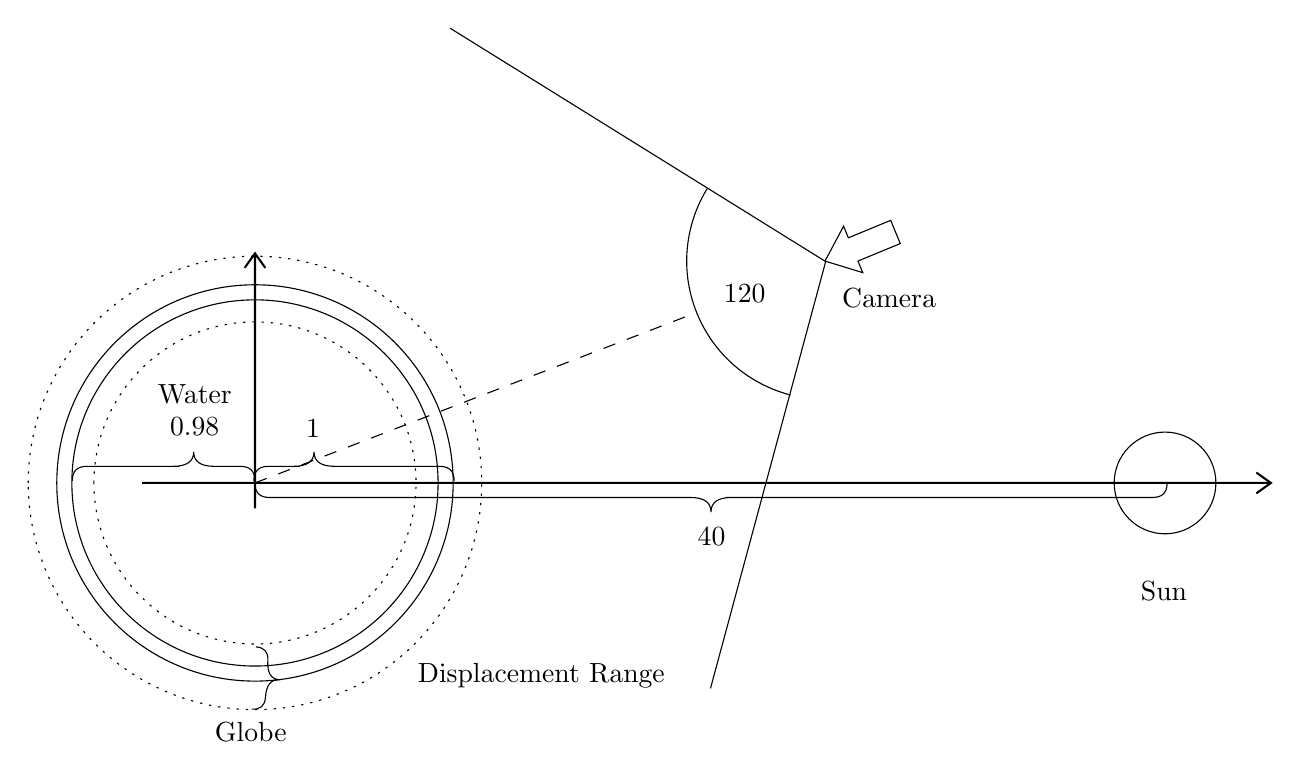
\begin{tikzpicture}[x=0.75pt,y=0.75pt,yscale=-1,xscale=1]
	%uncomment if require: \path (0,300); %set diagram left start at 0, and has height of 300

	%Shape: Circle [id:dp8728808526292304]
	\draw   (45.55,152) .. controls (45.55,99.27) and (88.3,56.52) .. (141.04,56.52) .. controls (193.77,56.52) and (236.52,99.27) .. (236.52,152) .. controls (236.52,204.73) and (193.77,247.48) .. (141.04,247.48) .. controls (88.3,247.48) and (45.55,204.73) .. (45.55,152) -- cycle ;
	%Shape: Circle [id:dp5674056113092418]
	\draw   (555,152) .. controls (555,138.47) and (565.97,127.5) .. (579.5,127.5) .. controls (593.03,127.5) and (604,138.47) .. (604,152) .. controls (604,165.53) and (593.03,176.5) .. (579.5,176.5) .. controls (565.97,176.5) and (555,165.53) .. (555,152) -- cycle ;
	%Shape: Axis 2D [id:dp667037457037013]
	\draw [line width=0.75]  (86.65,152) -- (630.5,152)(141.04,41.39) -- (141.04,164.29) (623.5,147) -- (630.5,152) -- (623.5,157) (136.04,48.39) -- (141.04,41.39) -- (146.04,48.39)  ;
	%Shape: Brace [id:dp5709274682232908]
	\draw   (141,152) .. controls (141,156.67) and (143.33,159) .. (148,159) -- (350.75,159) .. controls (357.42,159) and (360.75,161.33) .. (360.75,166) .. controls (360.75,161.33) and (364.08,159) .. (370.75,159)(367.75,159) -- (573.5,159) .. controls (578.17,159) and (580.5,156.67) .. (580.5,152) ;
	%Shape: Brace [id:dp38726825382608787]
	\draw   (237,151) .. controls (237,146.33) and (234.67,144) .. (230,144) -- (179.5,144) .. controls (172.83,144) and (169.5,141.67) .. (169.5,137) .. controls (169.5,141.67) and (166.17,144) .. (159.5,144)(162.5,144) -- (147.5,144) .. controls (142.83,144) and (140.5,146.33) .. (140.5,151) ;
	%Shape: Circle [id:dp559047975094662]
	\draw   (52.81,152) .. controls (52.81,103.28) and (92.31,63.78) .. (141.04,63.78) .. controls (189.76,63.78) and (229.26,103.28) .. (229.26,152) .. controls (229.26,200.72) and (189.76,240.22) .. (141.04,240.22) .. controls (92.31,240.22) and (52.81,200.72) .. (52.81,152) -- cycle ;
	%Shape: Brace [id:dp5585435570718464]
	\draw   (141,151) .. controls (141,146.33) and (138.67,144) .. (134,144) -- (121.5,144) .. controls (114.83,144) and (111.5,141.67) .. (111.5,137) .. controls (111.5,141.67) and (108.17,144) .. (101.5,144)(104.5,144) -- (60,144) .. controls (55.33,144) and (53,146.33) .. (53,151) ;
	%Left Arrow [id:dp007055379911458548]
	\draw   (415.67,45.1) -- (424.63,28.3) -- (426.94,33.9) -- (447.32,25.48) -- (451.94,36.67) -- (431.56,45.08) -- (433.87,50.68) -- cycle ;
	%Straight Lines [id:da28328227472011247]
	\draw  [dash pattern={on 4.5pt off 4.5pt}]  (141.04,152) -- (353.5,70) ;


	\draw   (235.08,-67.08) -- (416,45.34) -- (360.5,251) ;
	%Shape: Arc [id:dp11489271218380304]
	\draw  [draw opacity=0] (399.13,109.64) .. controls (379.34,104.55) and (362.14,90.46) .. (353.9,70.06) .. controls (345.66,49.66) and (348.24,27.59) .. (358.93,10.18) -- (415.67,45.1) -- cycle ; \draw   (399.13,109.64) .. controls (379.34,104.55) and (362.14,90.46) .. (353.9,70.06) .. controls (345.66,49.66) and (348.24,27.59) .. (358.93,10.18) ;
	%Shape: Circle [id:dp18625067716272725]
	\draw  [dash pattern={on 0.84pt off 2.51pt}] (31.79,152) .. controls (31.79,91.67) and (80.7,42.76) .. (141.04,42.76) .. controls (201.37,42.76) and (250.28,91.67) .. (250.28,152) .. controls (250.28,212.33) and (201.37,261.24) .. (141.04,261.24) .. controls (80.7,261.24) and (31.79,212.33) .. (31.79,152) -- cycle ;
	%Shape: Circle [id:dp21219909757761868]
	\draw  [dash pattern={on 0.84pt off 2.51pt}] (63.44,152) .. controls (63.44,109.15) and (98.18,74.41) .. (141.04,74.41) .. controls (183.89,74.41) and (218.63,109.15) .. (218.63,152) .. controls (218.63,194.85) and (183.89,229.59) .. (141.04,229.59) .. controls (98.18,229.59) and (63.44,194.85) .. (63.44,152) -- cycle ;
	%Shape: Brace [id:dp5998815658908982]
	\draw   (139.5,261) .. controls (143.62,261.27) and (145.82,259.35) .. (146.09,255.23) -- (146.09,255.23) .. controls (146.48,249.35) and (148.74,246.55) .. (152.85,246.82) .. controls (148.74,246.55) and (146.87,243.47) .. (147.26,237.59)(147.09,240.23) -- (147.26,237.59) .. controls (147.53,233.47) and (145.61,231.27) .. (141.5,231) ;

	% Text Node
	\draw (139,272) node  [align=left] {Globe};
	% Text Node
	\draw (579,204) node  [align=left] {Sun};
	% Text Node
	\draw (361,178) node  [align=left] {$40$};
	% Text Node
	\draw (169,126) node  [align=left] {$1$};
	% Text Node
	\draw (112,125) node  [align=left] {$0.98$};
	% Text Node
	\draw (112,109) node  [align=left] {Water};
	% Text Node
	\draw (446.5,63) node  [align=left] {Camera};
	% Text Node
	\draw (377,61) node  [align=left] {$120°$};
	% Text Node
	\draw (279,245) node  [align=left] {Displacement Range};


	\end{tikzpicture}


	\caption{A színpad elemei}
	\label{fig:stage-structure}
\end{figure}

\subsubsection{A felszín}

A felszín displacement mapja egy memóriában található canvas objektum amit textúraként használunk. A jobb hatás érdekében ezt bumb-mapként \cite{Bump} is használjuk. Egy projekt betöltésekor és minden további módosításkor ez a textúra az adatbázisból újra betöltődik. Mivel a textúránk egy canvas objektumon létezik, könnyen elérhetjük a canvas összes rajzfunkcióját, hogy egyszerűen, valós időben módosítsuk a térképet. A projekt szerkesztés menüjében lehetőségünk van bármikor betölteni bármilyen képet amit aztán ilyen textúraként fog használni az alkalmazás. Szerkesztésnél, minden, a bolygó felületén elhelyezkedő objektum megvizsgálja, hogy milyen magasan fog alatta vagy felette a displacement megjelenni. Ehhez is raycasting használunk, ahol a kemera helyett az adott objektumból a gömb közepe felé vetítünk egy sugarat. Ez a sugárvetés megmutatja, hogy a felület milyen $(u, v)$ pontján áll az adott objektum. Ezen ponton a textúra fényességét meg tudjuk vizsgálni, és kiszámolni az eltolás mértékét, ugyanúgy ahogy azt a renderer is fogja tenni. Ezzel biztosítva van, hogy minden felszíni elem látszik akkor is ha a displacement alapból eltakarná.

\subsubsection{A szereplők}

A felszíni objektumok nagyrészt szereplőkből állnak. Ők szintén gömbök, saját emisszív felülettel, hogy a bolygó sötét oldalán is könnyen látszódjanak. Rendelkeznek még két fajta körvonallal is ha az egér felettük helyezkedik el (vagy a hozzá tartozó, idővonalbeli sávja felett), vagy ki vannak választva.

Egy szereplő pontos pozíciójának meghatározásához a deltáit kell figyelembe vennünk. Az AVL fa implementáció amiben ezek el vannak helyezve rendelkezik olyan eljárással amivel nem fontos olyan kulcsot keresni ami tényleg létezik, mert a kulcshoz mindkét irányban legközelebb álló csomópontokkal fog visszatérni. Pontos egyezés esetén így mindkét csomópont ugyanaz lenne mint ha a hagyományos módon kértük volna le a kulcson található értéket.

A már meglévő csővezetékeink közzül a szereplők, a jelenlegi idő és az esetlegesen felülírt pozíciók csövét összevezetjük a \lstinline[columns=fixed]{combineLatest} operátorral. Emiatt a pozíciókat kiszámoló eljárás mindig le fog futni, ha a három közzül bármelyik is megváltozik, a másik kettő utolsó eredményével.

Az eljárás minden szereplőre, aszinkron módon történik egyszerre. A cél kiszámolni minden színész csoportjának kvaternióit\cite{Quaternion}, hogy megfelelően legyenek elforgatva.

\begin{algorithm}[H]
	\caption{Pozícionálás}
	\label{alg:ibb}
	\textbf{\underline{Subscription}} pos($A, C, O$), ahol $A$ a szereplő. $C$ az idő. $O$ a felülírások listája.
	\begin{algorithmic}[1] % sorszámok megjelenítése minden n. sor előtt, most n = 1
	\STATE $e$ := $C$ körüli delták.

	\IF[Ha vannak felülírások]{$O$}
		\FOR[A színész összes deltájára]{$d : A.deltas$}
			\FOR{$o : O$}
				\IF[Ha ehhez tartozik]{$d.time = o.time$}
					\STATE $d.time := d.newTime$
				\ENDIF
			\ENDFOR

			\IF{$d.time >= e[0].time \wedge d.time <= C$}
				\STATE $e[0] := d$
			\ENDIF
			\IF{$d.time <= e[1].time \wedge d.time >= C$}
				\STATE $e[1] := d$
			\ENDIF

		\ENDFOR
	\ENDIF

	\STATE $t := mapLinear(C, e[0].time, e[1].time, 0, 1)$
	\STATE $a := $A színész objektuma a színtéren.  \COMMENT{ID alapján.}
	\IF[Ha nem létezik, akkor itt létrehozzuk.]{!$a$}
		\STATE $a$ := Új színész objektum. \COMMENT{A színtérre is felkerül.}
	\ENDIF
	\STATE $angle := \angle(a.\overrightarrow{from}, a.\overrightarrow{to})$ \COMMENT{A cél és a forrás közötti távolság radiánban.}
	\STATE $\overrightarrow{norm} := a.\overrightarrow{from} × a.\overrightarrow{to}$ \COMMENT{A cél és a forrás normálvektora.}
	\STATE $\overrightarrow{result} := a.\overrightarrow{from}.applyAxisAngle(\overrightarrow{norm}, t * angle) $
	\STATE $a$.updateHeight() \COMMENT{A magasság korrigálása}
	\end{algorithmic}
\end{algorithm}


\subsection{Manipuláció}

A szereplők pozícióját itt a színtéren lehet megváltoztatni, viszont meg kell felelnünk egy nagyon fontos megszorításnak. A szereplő helyzete soha nem lehet olyan távol az előző és a következő helyzettől, hogy azt már képességeinek megfelelően ne tudja elérni.

Ahhoz hogy mindig a megfelelő területen tartsuk a szereplőt, azokban az esetekben amikor vagy a jövőben, vagy a múltban már nincs több esemény, elég az egyetlen környező esemény megengedett távolságán belül tartalni a szereplőt. Ha a kért pozíció távolsága kisebb mint a megengedett, a pozíciót rögzítjük. Ha nem, a legközelebb lévő pozíció lesz rögzítve ami még megengedett.

Abban az esetben ha két környező esemény van gyakorlatilag két, a gömbfelületen található kör metszetében keressük a legközelebbi pontot.

\begin{figure}[h!]
	\centering
	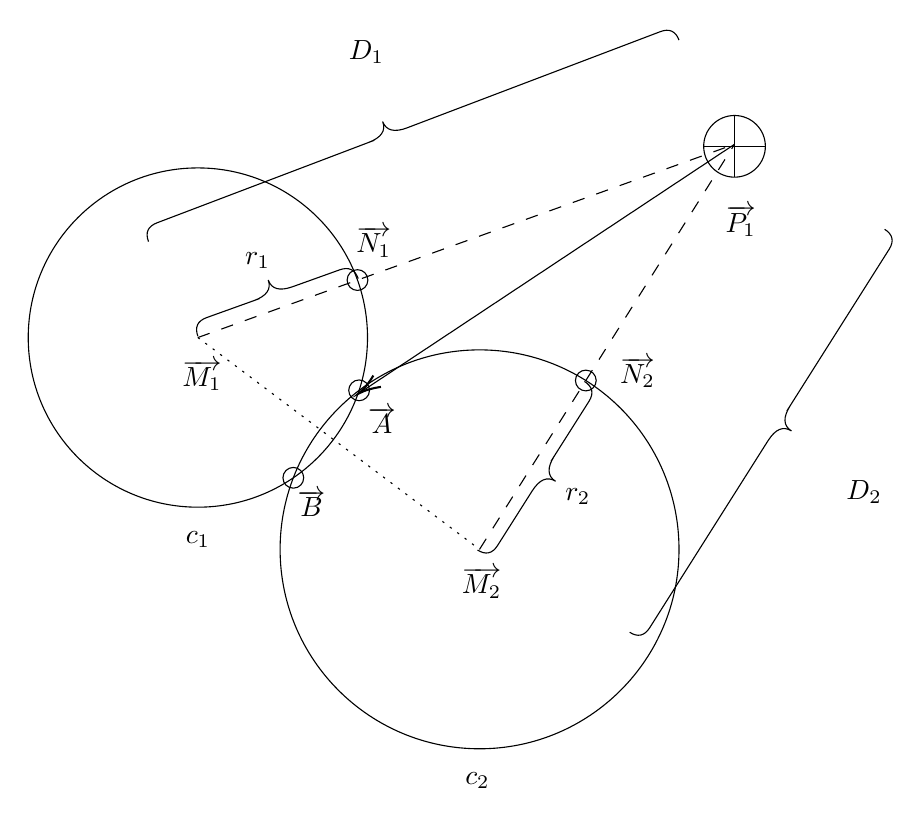
\begin{tikzpicture}[x=0.75pt,y=0.75pt,yscale=-1,xscale=1]
	%uncomment if require: \path (0,389); %set diagram left start at 0, and has height of 389

	%Shape: Circle [id:dp5885912263778241]
	\draw   (241.35,257.9) .. controls (241.35,204.83) and (284.38,161.81) .. (337.45,161.81) .. controls (390.52,161.81) and (433.54,204.83) .. (433.54,257.9) .. controls (433.54,310.97) and (390.52,354) .. (337.45,354) .. controls (284.38,354) and (241.35,310.97) .. (241.35,257.9) -- cycle ;
	%Shape: Ellipse [id:dp15448687207841338]
	\draw  [fill={rgb, 255:red, 255; green, 212; blue, 145 }  ,fill opacity=0 ] (120,155.87) .. controls (120,110.73) and (156.59,74.14) .. (201.73,74.14) .. controls (246.87,74.14) and (283.46,110.73) .. (283.46,155.87) .. controls (283.46,201) and (246.87,237.6) .. (201.73,237.6) .. controls (156.59,237.6) and (120,201) .. (120,155.87) -- cycle ;
	%Straight Lines [id:da6006500643796313]
	\draw  [dash pattern={on 0.84pt off 2.51pt}]  (201.73,155.87) -- (337.45,257.9) ;


	%Straight Lines [id:da5175683117647778]
	\draw  [dash pattern={on 4.5pt off 4.5pt}]  (201.73,155.87) -- (460.29,62.75) ;


	%Straight Lines [id:da33352637244621164]
	\draw  [dash pattern={on 4.5pt off 4.5pt}]  (337.45,257.9) -- (460.29,62.75) ;


	\draw   (445.43,63.74) .. controls (445.43,55.53) and (452.08,48.88) .. (460.29,48.88) .. controls (468.49,48.88) and (475.15,55.53) .. (475.15,63.74) .. controls (475.15,71.94) and (468.49,78.6) .. (460.29,78.6) .. controls (452.08,78.6) and (445.43,71.94) .. (445.43,63.74) -- cycle ; \draw   (445.43,63.74) -- (475.15,63.74) ; \draw   (460.29,48.88) -- (460.29,78.6) ;
	%Straight Lines [id:da19257704763660777]
	\draw    (460.29,62.75) -- (280.67,181.84) ;
	\draw [shift={(279,182.95)}, rotate = 326.45] [color={rgb, 255:red, 0; green, 0; blue, 0 }  ][line width=0.75]    (10.93,-3.29) .. controls (6.95,-1.4) and (3.31,-0.3) .. (0,0) .. controls (3.31,0.3) and (6.95,1.4) .. (10.93,3.29)   ;

	%Shape: Brace [id:dp007237602952800293]
	\draw   (279,127.47) .. controls (277.42,123.08) and (274.43,121.67) .. (270.04,123.25) -- (247.41,131.37) .. controls (241.14,133.62) and (237.21,132.55) .. (235.63,128.16) .. controls (237.21,132.55) and (234.86,135.88) .. (228.59,138.13)(231.41,137.12) -- (205.95,146.26) .. controls (201.56,147.83) and (200.15,150.82) .. (201.73,155.21) ;
	%Shape: Brace [id:dp7846975839966284]
	\draw   (336.46,258.23) .. controls (340.4,260.73) and (343.62,260.01) .. (346.12,256.07) -- (362.77,229.81) .. controls (366.34,224.18) and (370.09,222.62) .. (374.04,225.11) .. controls (370.09,222.62) and (369.91,218.55) .. (373.48,212.92)(371.87,215.45) -- (390.13,186.66) .. controls (392.63,182.72) and (391.91,179.5) .. (387.97,177) ;
	%Shape: Brace [id:dp41704229855363284]
	\draw   (433.54,12.55) .. controls (431.88,8.19) and (428.87,6.84) .. (424.51,8.5) -- (302.6,54.81) .. controls (296.37,57.18) and (292.42,56.18) .. (290.76,51.81) .. controls (292.42,56.18) and (290.13,59.54) .. (283.9,61.91)(286.71,60.84) -- (182.01,100.61) .. controls (177.65,102.27) and (176.3,105.28) .. (177.95,109.64) ;
	%Shape: Brace [id:dp09992687654682131]
	\draw   (409.76,297.86) .. controls (413.71,300.35) and (416.93,299.63) .. (419.42,295.69) -- (476.43,205.57) .. controls (480,199.94) and (483.75,198.37) .. (487.7,200.86) .. controls (483.75,198.37) and (483.56,194.3) .. (487.13,188.67)(485.52,191.2) -- (534.78,113.35) .. controls (537.27,109.41) and (536.55,106.19) .. (532.6,103.69) ;

	% Text Node
	\draw (203.71,174) node  [align=left] {$\overrightarrow{M_1}$};
	% Text Node
	\draw (338.44,274.05) node  [align=left] {$\overrightarrow{M_2}$};
	% Text Node
	\draw (230.48,118.73) node  [align=left] {$r_1$};
	% Text Node
	\draw (384.8,232.36) node  [align=left] {$r_2$};
	% Text Node
	\draw (201.78,253.22) node  [align=left] {$c_1$};
	% Text Node
	\draw (336.44,369.17) node  [align=left] {$c_2$};
	% Text Node
	\draw (463.26,99.73) node  [align=left] {$\overrightarrow{P_1}$};
	% Text Node
	\draw (282.96,18.5) node  [align=left] {$D_1$};
	% Text Node
	\draw (522.7,230.5) node  [align=left] {$D_2$};
	% Text Node
	\draw (286.48,109.73) node  [align=left] {$\overrightarrow{N_1}$};
	% Text Node
	\draw (413.48,172.73) node  [align=left] {$\overrightarrow{N_2}$};
	% Text Node
	\draw (290.48,195.73) node  [align=left] {$\overrightarrow{A}$};
	% Text Node
	\draw (256.48,235.73) node  [align=left] {$\overrightarrow{B}$};

	\draw   (279.42, 181.3) circle [x radius= 5, y radius= 5]   ;
	\draw   (247.72, 223.44) circle [x radius= 5, y radius= 5]   ;
	\draw   (388.64, 176.57) circle [x radius= 5, y radius= 5]   ;
	\draw   (278.64, 128.17) circle [x radius= 5, y radius= 5]   ;
	\end{tikzpicture}
\caption{Körök metszete gömbfelületen}
\label{fig:spherical-sphere-intersection}
\end{figure}

\begin{tabular}{@{}ll@{}}
	\textbf{Jel} & \textbf{Leírás} \\
	$\overrightarrow{M_1}$ & Előző pozíció \\
	$\overrightarrow{M_2}$ & Következő pozíció \\
	$r_1$ & A jelenlegi időpont és $\overrightarrow{M_1}$ időpontja között maximálisan megtehető út \\
	$r_2$ & A jelenlegi időpont és $\overrightarrow{M_2}$ időpontja között maximálisan megtehető út \\
	$\overrightarrow{c_1}$ & $\overrightarrow{M_1}$ és $r_1$ által alkotott kör a gömbfelületen \\
	$\overrightarrow{c_2}$ & $\overrightarrow{M_2}$ és $r_2$ által alkotott kör a gömbfelületen \\
	$\overrightarrow{P_1}$ & A felhasználó által kiválaszott célpozíció \\
	$D_1$ & A gömbfelületen vett távolság $\overrightarrow{P_1}$ és $\overrightarrow{M_1}$ között \\
	$D_2$ & A gömbfelületen vett távolság $\overrightarrow{P_1}$ és $\overrightarrow{M_2}$ között \\
	$\overrightarrow{N_1}$ & A gömbfelület $\overrightarrow{M_1}$ és $\overrightarrow{P_1}$ pont által meghatározott \\
	& főkörén az a pont amely pontosan $r_1$ távolságra van $\overrightarrow{M_1}$-től \\
	$\overrightarrow{N_2}$ & A gömbfelület $\overrightarrow{M_2}$ és $\overrightarrow{P_1}$ pont által meghatározott \\
	& főkörén az a pont amely pontosan $r_2$ távolságra van $\overrightarrow{M_2}$-től \\
	$\overrightarrow{A}$ & $c_1$ és $c_2$ kör egyik metszéspontja \\
	$\overrightarrow{B}$ & $c_1$ és $c_2$ kör másik metszéspontja \\
	& \\
\end{tabular}

Ebben (\ref{fig:spherical-sphere-intersection}) az esetben a szereplő nem teljes sebességgel haladt a két pont között ezért ha félúton manipuláljuk, azt látjuk, hogy amellett, hogy mindkét ponthoz még eltudunk jutni, még van egy kis mozgásterünk ahol ugyanúgy eljutna a megadott időn belül $\overrightarrow{M_1}$-be és $\overrightarrow{M_2}$-be is képességeinek megfelelően. Meg kell határoznunk manipulálás közben, hogy $c_1$ és $c_2$ metszetében melyik pont van $\overrightarrow{P_1}$ ponthoz a legközelebb.

Manipulálás kezdetekor válnak elérhetővé a kellő információk $c_1$ és $c_2$ adatainak a kiszámolásához. Ekkor számoljuk ki $\overrightarrow{A}$ és $\overrightarrow{B}$ pontot is. Ezt manipulálásonként csak egyszer számoljuk ki. Ekkor helyezzük el a két indikátor gömbcikket. A végén pedig el lesznek rejtve. Manipulálás közben pedig folyamatosan számljuk a legközelebbi pont függvényét. A két gömbcikk overdraw módban kerül rajzolásra így el lehet őket helyezni pontosan a bolygó eredeti 1 sugarú felületére és úgy is mindig látszódni fognak. Sajnos nagyon eltérő displacement és alacsony szögből való megtekintés esetén kicsit csalóka lehet a grafika mivel a szereplők objektuma az eltolást figyelembe veszik. Ez viszont nem bizonyult túl zavarónak tesztelés közben.

\subsubsection{Azonos sugarú gömbcikkek metszésponjai}

$\overrightarrow{M_1}$ és $\overrightarrow{M_2}$ világ pozíciók, és mivel a bolygó centruma a $(0, 0, 0)$ pontban helyezkedik el, ezért ezek egyben geocentrikus pontok is. A problémát átfogalmazhatjuk egy egyszerűbb problémává. Ha keresünk az $\overrightarrow{M_1}$ és az origó által meghatározott vonalon egy pontot -- legyen $\overrightarrow{a}$ -- és sugarat amivel egy akkora gömböt képez ami pontosan a $c_1$ körön metszi a bolygó gömbjét, és analóg módon $\overrightarrow{M_2}$-höz egy $\overrightarrow{b}$ pontot és sugarat. Akkor az $\overrightarrow{a}$ pont $c_1$ körrel és $\overrightarrow{b}$ pont $c_2$ körrel egy-egy síkot határoznak meg, melyek metszésvonalán fog elhelyezkedni $\overrightarrow{A}$ és $\overrightarrow{B}$ pont is. Így a problémánk egy kör és egy egyenes metszetére redukálódott le.

\begin{figure}[h!]
	\centering

	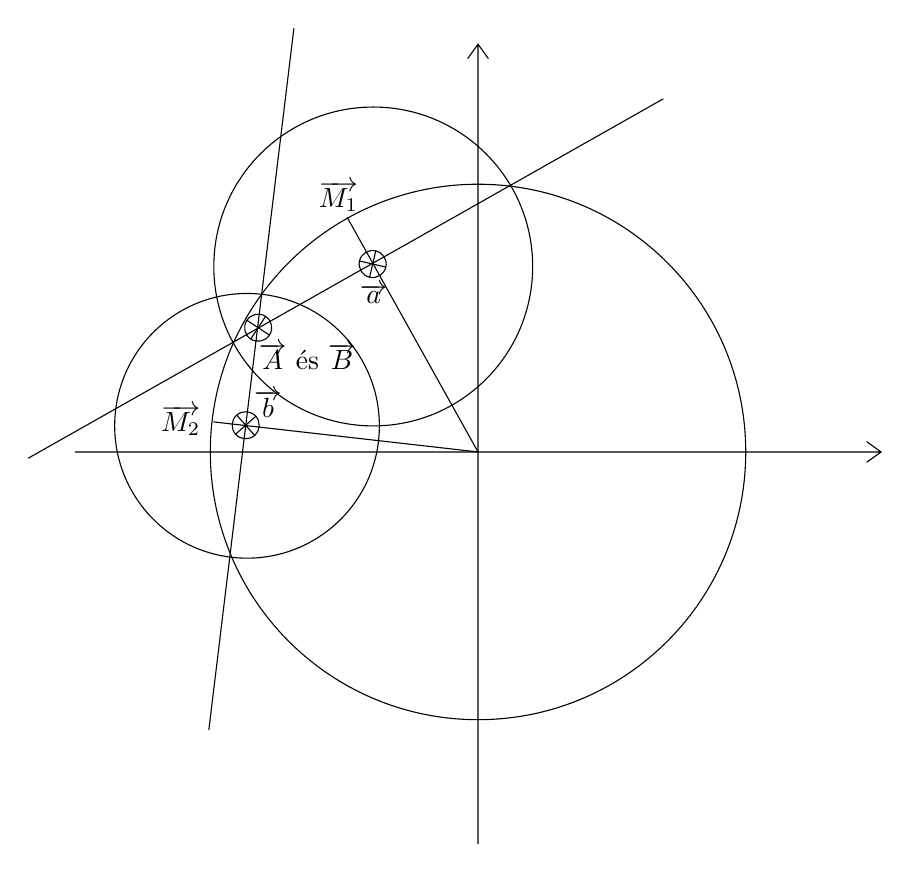
\begin{tikzpicture}[x=0.75pt,y=0.75pt,yscale=-1,xscale=1]
	%uncomment if require: \path (0,468); %set diagram left start at 0, and has height of 468

	%Shape: Circle [id:dp2263468573456704]
	\draw   (197.22,233.48) .. controls (197.22,162.24) and (254.97,104.49) .. (326.21,104.49) .. controls (397.44,104.49) and (455.19,162.24) .. (455.19,233.48) .. controls (455.19,304.72) and (397.44,362.47) .. (326.21,362.47) .. controls (254.97,362.47) and (197.22,304.72) .. (197.22,233.48) -- cycle ;
	%Shape: Circle [id:dp8130162816265305]
	\draw   (198.91,144.12) .. controls (198.91,101.69) and (233.3,67.3) .. (275.73,67.3) .. controls (318.15,67.3) and (352.54,101.69) .. (352.54,144.12) .. controls (352.54,186.54) and (318.15,220.93) .. (275.73,220.93) .. controls (233.3,220.93) and (198.91,186.54) .. (198.91,144.12) -- cycle ;
	%Shape: Circle [id:dp9863650593943492]
	\draw   (151.15,220.88) .. controls (151.15,185.67) and (179.7,157.12) .. (214.91,157.12) .. controls (250.13,157.12) and (278.68,185.67) .. (278.68,220.88) .. controls (278.68,256.1) and (250.13,284.65) .. (214.91,284.65) .. controls (179.7,284.65) and (151.15,256.1) .. (151.15,220.88) -- cycle ;
	%Straight Lines [id:da8253130424028727]
	\draw    (198.67,218.99) -- (326.21,233.48) ;


	%Straight Lines [id:da6219323829844645]
	\draw    (326.21,233.48) -- (263.16,120.43) ;


	%Shape: Axis 2D [id:dp7403279305833326]
	\draw  (132,233.48) -- (520.41,233.48)(326.21,37) -- (326.21,422.25) (513.41,228.48) -- (520.41,233.48) -- (513.41,238.48) (321.21,44) -- (326.21,37) -- (331.21,44)  ;
	\draw   (269.1,141.46) .. controls (269.92,137.95) and (273.43,135.77) .. (276.94,136.59) .. controls (280.44,137.41) and (282.62,140.92) .. (281.8,144.42) .. controls (280.98,147.93) and (277.48,150.11) .. (273.97,149.29) .. controls (270.46,148.47) and (268.28,144.96) .. (269.1,141.46) -- cycle ; \draw   (269.1,141.46) -- (281.8,144.42) ; \draw   (276.94,136.59) -- (273.97,149.29) ;
	\draw   (209.39,224.92) .. controls (207,222.22) and (207.26,218.1) .. (209.96,215.72) .. controls (212.66,213.34) and (216.78,213.59) .. (219.17,216.29) .. controls (221.55,218.99) and (221.29,223.12) .. (218.59,225.5) .. controls (215.89,227.88) and (211.77,227.62) .. (209.39,224.92) -- cycle ; \draw   (209.39,224.92) -- (219.17,216.29) ; \draw   (209.96,215.72) -- (218.59,225.5) ;
	%Straight Lines [id:da08394559625180209]
	\draw    (237.5,29.33) -- (196.5,367.5) ;


	%Straight Lines [id:da6409389593213928]
	\draw    (415.5,63.33) -- (109.5,236.5) ;


	\draw   (216.72,179.07) .. controls (213.7,177.11) and (212.85,173.06) .. (214.81,170.05) .. controls (216.78,167.03) and (220.82,166.18) .. (223.84,168.15) .. controls (226.86,170.11) and (227.71,174.15) .. (225.74,177.17) .. controls (223.77,180.19) and (219.73,181.04) .. (216.72,179.07) -- cycle ; \draw   (216.72,179.07) -- (223.84,168.15) ; \draw   (214.81,170.05) -- (225.74,177.17) ;

	% Text Node
	\draw (259,110.25) node  [align=left] {$\overrightarrow{M_1}$};
	% Text Node
	\draw (183,218.25) node  [align=left] {$\overrightarrow{M_2}$};
	% Text Node
	\draw (276,157.25) node  [align=left] {$\overrightarrow{a}$};
	% Text Node
	\draw (225,210.25) node  [align=left] {$\overrightarrow{b}$};
	% Text Node
	\draw (244,187.25) node  [align=left] {$\overrightarrow{A}$ és $\overrightarrow{B}$};

	\end{tikzpicture}
\caption{Az átfogalmazott példa, a két egyenes egy egy síkot jelölnek.}
\label{fig:three-sphere-intersection}
\end{figure}



\begin{algorithm}[H]
	\caption{Két kör metszéspontjai gömbfelületen}
	\label{alg:intersection}
	\textbf{\underline{Function}} intersection($\overrightarrow{M_1}, \overrightarrow{M_2}, r_1, r_2, R$) ahol $R$ a bolygó sugara kilóméterben
	\begin{algorithmic}[1]
	\STATE $\overrightarrow{x_1} := \overrightarrow{M_1}$ normalizálva \COMMENT{Valójában $\overrightarrow{M_1}$ és $\overrightarrow{M_2}$ vektor hossza már eleve 1}
	\STATE $\overrightarrow{x_2} := \overrightarrow{M_2}$ normalizálva
	\STATE $rad_1 := r_1 / R$ \COMMENT{Átváltás radiánba}
	\STATE $rad_2 := r_2 / R$
	\STATE $q := \overrightarrow{x_1} \bullet \overrightarrow{x_2}$ \COMMENT{A két vektor skaláris szorzata}
	\IF{$q^2 = 1$}
		\STATE return \COMMENT{A két kör nem metszheti egymást mert $\overrightarrow{M_1} = \overrightarrow{M_2}$  vagy $\overrightarrow{M_1}$ és $\overrightarrow{M_2}$ a centrumhoz képest a szemközti oldalon állnak. Ebben az esetben vagy a körök minden pontja metszi egymást, vagy egy sem.}
	\ENDIF
	\STATE $a := \frac{cos(rad_1) - q \cdot cos(rad_2)}{1 - q^2}$
	\STATE $b := \frac{cos(rad_2) - q \cdot cos(rad_1)}{1 - q^2}$
	\STATE $\overrightarrow{x_0} := \overrightarrow{x_1} \cdot a + \overrightarrow{x_2} \cdot b$
	\IF{$\overrightarrow{x_0}^2 > 1$}
		\STATE return \COMMENT{A két kör nem érintkezik.}
	\ENDIF
	\STATE $\overrightarrow{n} := \overrightarrow{x_1} × \overrightarrow{x_2}$
	\IF{$\overrightarrow{n}^2 = 0$}
		\STATE return \COMMENT{A két kör középpontja vagy megegyezik vagy szemközt állnak.}
	\ENDIF
	\STATE $t := \sqrt{ \frac{1 - \overrightarrow{x_0} \bullet \overrightarrow{x_0}}{\overrightarrow{n}^2}}$
	\STATE $\overrightarrow{i_0} := \overrightarrow{x_0} + \overrightarrow{n} \cdot t$
	\IF[Több eredmény csak pozitív $t$ esetén lehetséges]{$t > 0$}
		\STATE $\overrightarrow{i_1} := \overrightarrow{x_0} + \overrightarrow{n} \cdot -t$
		\STATE return [$\overrightarrow{i_0}$, $\overrightarrow{i_1}$]
	\ELSE
		\STATE return [$\overrightarrow{i_0}$]
	\ENDIF
	\end{algorithmic}
\end{algorithm}

\subsubsection{Körívek metszete gömbfelületen}

A legközelebbi pontok lehetnek $\overrightarrow{N_1}$, $\overrightarrow{N_2}$, $\overrightarrow{A}$ és $\overrightarrow{B}$. $\overrightarrow{N_1}$ és $\overrightarrow{N_2}$ viszont nem feltétlen helyezkednek el a metszés körívén. $\overrightarrow{N_1}$ és $\overrightarrow{N_2}$ akkor lesz érvényes, ha az adott $\overrightarrow{M}$ és $\overrightarrow{P}$ pont által meghatározott körív metszi az $\overrightarrow{A}$ és $\overrightarrow{B}$ által rajzolt körívet.

A \ref{fig:nearest-circle-intersection-examples}-es ábrán a $\overrightarrow{P_0}$ szerű pontok megfelelnek mindkét kitételnek -- mindkét ponthoz szükséges távolságon belül állnak -- így további dolgunk nincs velük. A $\overrightarrow{P_1}$ szerű pontok csak egy feltételnek felelnek meg. Az ő esetükben csak a másik kör középpontja felé forgatnunk a pozícióját, az $\overrightarrow{M_1} × \overrightarrow{P_1}$ tengelyen. A $\overrightarrow{P_2}$ és $\overrightarrow{P_3}$ pontok közötti különbség, hogy $\overrightarrow{P_2}$-nél a legközelebbi pont maga a metszés mert se $\overrightarrow{N_1}$ sem pedig $\overrightarrow{N_2}$ nem a megfelelő köríven helyezkedik el ilyen esetben.

\begin{figure}[h!]
	\centering
	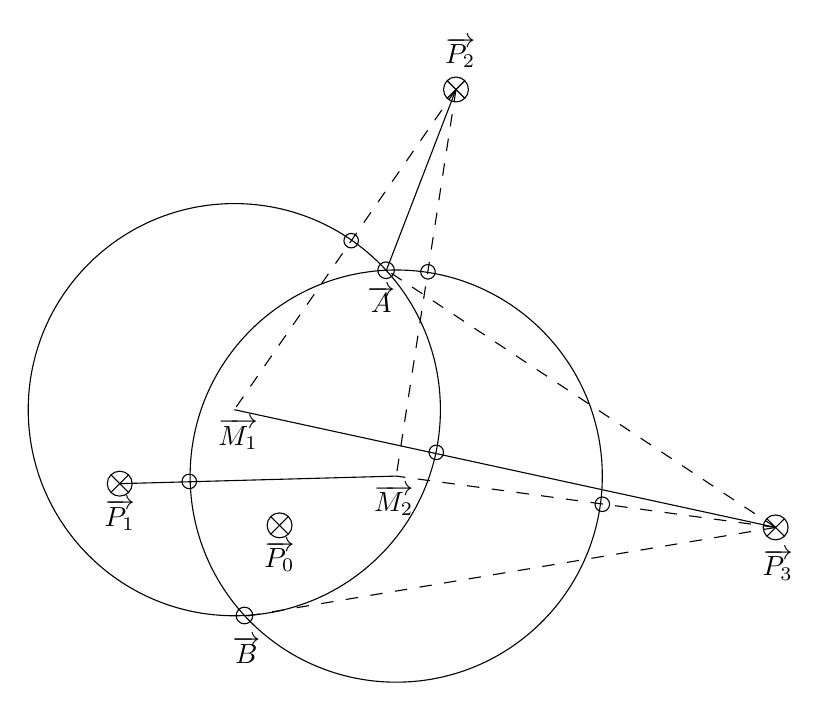
\begin{tikzpicture}[x=0.75pt,y=0.75pt,yscale=-1,xscale=1]
	%uncomment if require: \path (0,468); %set diagram left start at 0, and has height of 468

	%Shape: Circle [id:dp8166187689889921]
	\draw   (134.91,201.6) .. controls (134.91,146.76) and (179.37,102.3) .. (234.21,102.3) .. controls (289.05,102.3) and (333.5,146.76) .. (333.5,201.6) .. controls (333.5,256.43) and (289.05,300.89) .. (234.21,300.89) .. controls (179.37,300.89) and (134.91,256.43) .. (134.91,201.6) -- cycle ;
	%Shape: Circle [id:dp6909695032298264]
	\draw   (212.91,233.6) .. controls (212.91,178.76) and (257.37,134.3) .. (312.21,134.3) .. controls (367.05,134.3) and (411.5,178.76) .. (411.5,233.6) .. controls (411.5,288.43) and (367.05,332.89) .. (312.21,332.89) .. controls (257.37,332.89) and (212.91,288.43) .. (212.91,233.6) -- cycle ;
	%Flowchart: Summing Junction [id:dp009162364923596789]
	\draw   (250,257.33) .. controls (250,254.02) and (252.69,251.33) .. (256,251.33) .. controls (259.31,251.33) and (262,254.02) .. (262,257.33) .. controls (262,260.65) and (259.31,263.33) .. (256,263.33) .. controls (252.69,263.33) and (250,260.65) .. (250,257.33) -- cycle ; \draw   (251.76,253.09) -- (260.24,261.58) ; \draw   (260.24,253.09) -- (251.76,261.58) ;
	%Flowchart: Summing Junction [id:dp17652291932752062]
	\draw   (173,237.25) .. controls (173,233.94) and (175.69,231.25) .. (179,231.25) .. controls (182.31,231.25) and (185,233.94) .. (185,237.25) .. controls (185,240.56) and (182.31,243.25) .. (179,243.25) .. controls (175.69,243.25) and (173,240.56) .. (173,237.25) -- cycle ; \draw   (174.76,233.01) -- (183.24,241.49) ; \draw   (183.24,233.01) -- (174.76,241.49) ;
	%Flowchart: Summing Junction [id:dp4645172529660282]
	\draw   (489,258.33) .. controls (489,255.02) and (491.69,252.33) .. (495,252.33) .. controls (498.31,252.33) and (501,255.02) .. (501,258.33) .. controls (501,261.65) and (498.31,264.33) .. (495,264.33) .. controls (491.69,264.33) and (489,261.65) .. (489,258.33) -- cycle ; \draw   (490.76,254.09) -- (499.24,262.58) ; \draw   (499.24,254.09) -- (490.76,262.58) ;
	%Flowchart: Summing Junction [id:dp5476818076821499]
	\draw   (335,47.33) .. controls (335,44.02) and (337.69,41.33) .. (341,41.33) .. controls (344.31,41.33) and (347,44.02) .. (347,47.33) .. controls (347,50.65) and (344.31,53.33) .. (341,53.33) .. controls (337.69,53.33) and (335,50.65) .. (335,47.33) -- cycle ; \draw   (336.76,43.09) -- (345.24,51.58) ; \draw   (345.24,43.09) -- (336.76,51.58) ;
	%Straight Lines [id:da49460456729427316]
	\draw  [dash pattern={on 4.5pt off 4.5pt}]  (341,47.33) -- (234.21,201.6) ;


	%Straight Lines [id:da9864649930793872]
	\draw  [dash pattern={on 4.5pt off 4.5pt}]  (341,47.33) -- (312.21,233.6) ;


	%Straight Lines [id:da1538944910181792]
	\draw    (341,47.33) -- (307.5,134.33) ;


	%Flowchart: Connector [id:dp7527304205187331]
	\draw   (324,135.17) .. controls (324,133.23) and (325.57,131.67) .. (327.5,131.67) .. controls (329.43,131.67) and (331,133.23) .. (331,135.17) .. controls (331,137.1) and (329.43,138.67) .. (327.5,138.67) .. controls (325.57,138.67) and (324,137.1) .. (324,135.17) -- cycle ;
	%Flowchart: Connector [id:dp27712539160217364]
	\draw   (287,120.17) .. controls (287,118.23) and (288.57,116.67) .. (290.5,116.67) .. controls (292.43,116.67) and (294,118.23) .. (294,120.17) .. controls (294,122.1) and (292.43,123.67) .. (290.5,123.67) .. controls (288.57,123.67) and (287,122.1) .. (287,120.17) -- cycle ;
	%Straight Lines [id:da2513261195102452]
	\draw    (495,258.33) -- (234.21,201.6) ;


	%Flowchart: Connector [id:dp778704099897711]
	\draw   (328,222.17) .. controls (328,220.23) and (329.57,218.67) .. (331.5,218.67) .. controls (333.43,218.67) and (335,220.23) .. (335,222.17) .. controls (335,224.1) and (333.43,225.67) .. (331.5,225.67) .. controls (329.57,225.67) and (328,224.1) .. (328,222.17) -- cycle ;
	%Straight Lines [id:da16321655779119704]
	\draw  [dash pattern={on 4.5pt off 4.5pt}]  (495,258.33) -- (312.21,233.6) ;


	%Flowchart: Connector [id:dp00875038400506023]
	\draw   (408,247.17) .. controls (408,245.23) and (409.57,243.67) .. (411.5,243.67) .. controls (413.43,243.67) and (415,245.23) .. (415,247.17) .. controls (415,249.1) and (413.43,250.67) .. (411.5,250.67) .. controls (409.57,250.67) and (408,249.1) .. (408,247.17) -- cycle ;
	%Straight Lines [id:da46001771981700856]
	\draw  [dash pattern={on 4.5pt off 4.5pt}]  (495,258.33) -- (307.5,134.33) ;


	%Straight Lines [id:da4073168758118153]
	\draw  [dash pattern={on 4.5pt off 4.5pt}]  (495,258.33) -- (239,301.25) ;


	%Straight Lines [id:da30499884455793724]
	\draw    (179,237.25) -- (312.21,233.6) ;


	%Flowchart: Connector [id:dp8279616571890565]
	\draw   (209,236.17) .. controls (209,234.23) and (210.57,232.67) .. (212.5,232.67) .. controls (214.43,232.67) and (216,234.23) .. (216,236.17) .. controls (216,238.1) and (214.43,239.67) .. (212.5,239.67) .. controls (210.57,239.67) and (209,238.1) .. (209,236.17) -- cycle ;

	% Text Node
	\draw (305,148.33) node  [align=left] {$\overrightarrow{A}$};
	% Text Node
	\draw (240,317.33) node  [align=left] {$\overrightarrow{B}$};
	% Text Node
	\draw (236,213.33) node  [align=left] {$\overrightarrow{M_1}$};
	% Text Node
	\draw (311,245.33) node  [align=left] {$\overrightarrow{M_2}$};
	% Text Node
	\draw (343,29.33) node  [align=left] {$\overrightarrow{P_2}$};
	% Text Node
	\draw (496,276.33) node  [align=left] {$\overrightarrow{P_3}$};
	% Text Node
	\draw (256,272.33) node  [align=left] {$\overrightarrow{P_0}$};
	% Text Node
	\draw (179,252.33) node  [align=left] {$\overrightarrow{P_1}$};

	\draw   (307.33, 134.42) circle [x radius= 4, y radius= 4]   ;
	\draw   (239.09, 300.77) circle [x radius= 4, y radius= 4]   ;
	\end{tikzpicture}

\caption{Különböző esetek a legközelebbi pontok esetében}
\label{fig:nearest-circle-intersection-examples}
\end{figure}

\pagebreak

Miután megvan $\overrightarrow{A}$, $\overrightarrow{B}$, $\overrightarrow{N_1}$ és $\overrightarrow{N_2}$, el kell tudnunk dönteni, hogy $\overrightarrow{N_1}$ és $\overrightarrow{N_2}$ a megfelelő köríven vannak e. A three.js könyvtár egyszerű eszközöket ad arra, hogy két vektor bezárt szögét kiszámoljuk.

$$\overrightarrow{M_1A} := \overrightarrow{M_1} - \overrightarrow{A}$$
$$\overrightarrow{M_1B} := \overrightarrow{M_1} - \overrightarrow{B}$$
$$\overrightarrow{M_1N_1} := \overrightarrow{M_1} - \overrightarrow{N_1}$$

 Ha $\angle(\overrightarrow{M_1A}, \overrightarrow{M_1B}) - \angle(\overrightarrow{M_1A}, \overrightarrow{M_1N_1}) + \angle(\overrightarrow{M_1B}, \overrightarrow{M_1N_1}) \ge 0$ akkor tudjuk, hogy a nagyobb köríven áll $\overrightarrow{N_1}$.

\begin{figure}[h!]
	\centering

	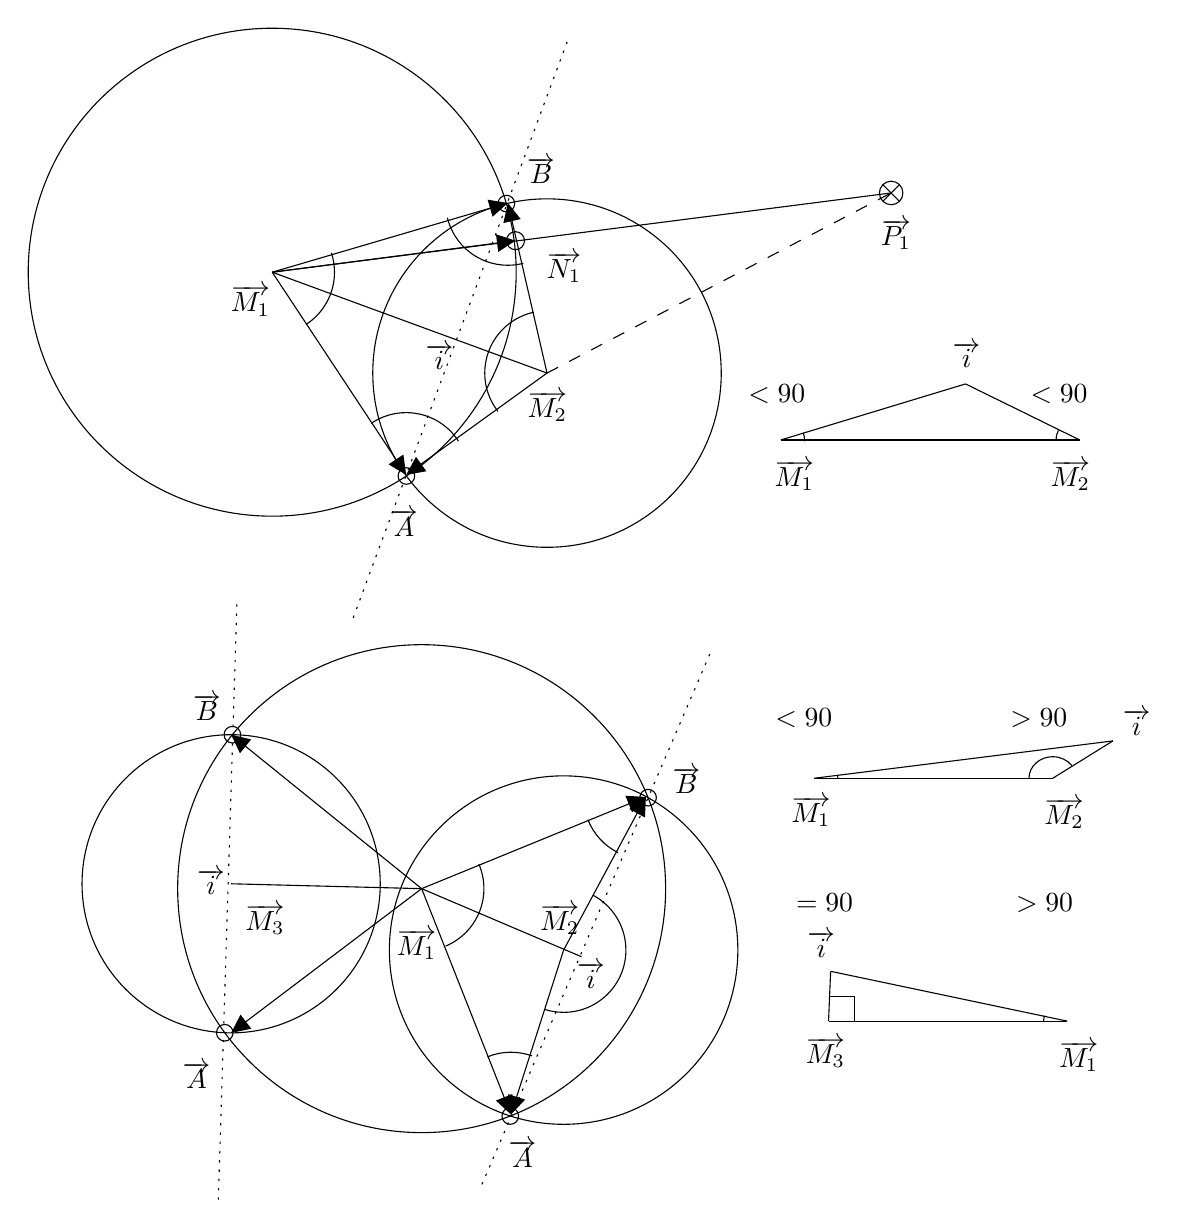
\begin{tikzpicture}[x=0.75pt,y=0.75pt,yscale=-1,xscale=1]
	%uncomment if require: \path (0,1036.3333435058594); %set diagram left start at 0, and has height of 1036.3333435058594

	%Shape: Circle [id:dp7147274460574649]
	\draw   (71.91,135.85) .. controls (71.91,70.93) and (124.54,18.3) .. (189.46,18.3) .. controls (254.37,18.3) and (307,70.93) .. (307,135.85) .. controls (307,200.76) and (254.37,253.39) .. (189.46,253.39) .. controls (124.54,253.39) and (71.91,200.76) .. (71.91,135.85) -- cycle ;
	%Shape: Circle [id:dp10982270342140565]
	\draw   (237.91,184.44) .. controls (237.91,138.08) and (275.5,100.5) .. (321.86,100.5) .. controls (368.22,100.5) and (405.8,138.08) .. (405.8,184.44) .. controls (405.8,230.81) and (368.22,268.39) .. (321.86,268.39) .. controls (275.5,268.39) and (237.91,230.81) .. (237.91,184.44) -- cycle ;
	%Straight Lines [id:da14970762671387594]
	\draw    (189.46,135.85) -- (321.86,184.44) ;


	%Straight Lines [id:da5018657633210779]
	\draw    (189.46,135.85) -- (301.08,103.06) ;
	\draw [shift={(303,102.5)}, rotate = 523.63] [fill={rgb, 255:red, 0; green, 0; blue, 0 }  ][line width=0.75]  [draw opacity=0] (8.93,-4.29) -- (0,0) -- (8.93,4.29) -- cycle    ;

	%Straight Lines [id:da8787252418767009]
	\draw    (189.46,135.85) -- (252.9,231.83) ;
	\draw [shift={(254,233.5)}, rotate = 236.54] [fill={rgb, 255:red, 0; green, 0; blue, 0 }  ][line width=0.75]  [draw opacity=0] (8.93,-4.29) -- (0,0) -- (8.93,4.29) -- cycle    ;

	%Straight Lines [id:da334184052442988]
	\draw    (303.45,104.45) -- (321.86,184.44) ;

	\draw [shift={(303,102.5)}, rotate = 77.04] [fill={rgb, 255:red, 0; green, 0; blue, 0 }  ][line width=0.75]  [draw opacity=0] (8.93,-4.29) -- (0,0) -- (8.93,4.29) -- cycle    ;
	%Straight Lines [id:da5281291307703042]
	\draw    (255.62,232.33) -- (321.86,184.44) ;

	\draw [shift={(254,233.5)}, rotate = 324.14] [fill={rgb, 255:red, 0; green, 0; blue, 0 }  ][line width=0.75]  [draw opacity=0] (8.93,-4.29) -- (0,0) -- (8.93,4.29) -- cycle    ;
	%Shape: Circle [id:dp8204009048923462]
	\draw   (143.91,432.85) .. controls (143.91,367.93) and (196.54,315.3) .. (261.46,315.3) .. controls (326.37,315.3) and (379,367.93) .. (379,432.85) .. controls (379,497.76) and (326.37,550.39) .. (261.46,550.39) .. controls (196.54,550.39) and (143.91,497.76) .. (143.91,432.85) -- cycle ;
	%Shape: Circle [id:dp5891184045449915]
	\draw   (245.91,462.44) .. controls (245.91,416.08) and (283.5,378.5) .. (329.86,378.5) .. controls (376.22,378.5) and (413.8,416.08) .. (413.8,462.44) .. controls (413.8,508.81) and (376.22,546.39) .. (329.86,546.39) .. controls (283.5,546.39) and (245.91,508.81) .. (245.91,462.44) -- cycle ;
	%Straight Lines [id:da7300207606590179]
	\draw    (261.46,432.85) -- (338.5,465.67) ;


	%Straight Lines [id:da7866363401157963]
	\draw    (261.46,432.85) -- (367.65,389.42) ;
	\draw [shift={(369.5,388.67)}, rotate = 517.76] [fill={rgb, 255:red, 0; green, 0; blue, 0 }  ][line width=0.75]  [draw opacity=0] (8.93,-4.29) -- (0,0) -- (8.93,4.29) -- cycle    ;

	%Straight Lines [id:da5973975562618397]
	\draw    (261.46,432.85) -- (303.76,539.81) ;
	\draw [shift={(304.5,541.67)}, rotate = 248.42000000000002] [fill={rgb, 255:red, 0; green, 0; blue, 0 }  ][line width=0.75]  [draw opacity=0] (8.93,-4.29) -- (0,0) -- (8.93,4.29) -- cycle    ;

	%Straight Lines [id:da44579030739359893]
	\draw    (368.55,390.43) -- (329.86,462.44) ;

	\draw [shift={(369.5,388.67)}, rotate = 118.25] [fill={rgb, 255:red, 0; green, 0; blue, 0 }  ][line width=0.75]  [draw opacity=0] (8.93,-4.29) -- (0,0) -- (8.93,4.29) -- cycle    ;
	%Straight Lines [id:da42826623065586467]
	\draw    (305.11,539.76) -- (329.86,462.44) ;

	\draw [shift={(304.5,541.67)}, rotate = 287.75] [fill={rgb, 255:red, 0; green, 0; blue, 0 }  ][line width=0.75]  [draw opacity=0] (8.93,-4.29) -- (0,0) -- (8.93,4.29) -- cycle    ;
	%Shape: Arc [id:dp2161098265865362]
	\draw  [draw opacity=0] (289.03,421.01) .. controls (290.59,424.64) and (291.46,428.64) .. (291.46,432.85) .. controls (291.46,445.31) and (283.85,456) .. (273.03,460.53) -- (261.46,432.85) -- cycle ; \draw   (289.03,421.01) .. controls (290.59,424.64) and (291.46,428.64) .. (291.46,432.85) .. controls (291.46,445.31) and (283.85,456) .. (273.03,460.53) ;
	%Shape: Arc [id:dp37186414101113785]
	\draw  [draw opacity=0] (298.2,202.89) .. controls (294.23,197.81) and (291.86,191.4) .. (291.86,184.44) .. controls (291.86,170.06) and (301.98,158.05) .. (315.48,155.12) -- (321.86,184.44) -- cycle ; \draw   (298.2,202.89) .. controls (294.23,197.81) and (291.86,191.4) .. (291.86,184.44) .. controls (291.86,170.06) and (301.98,158.05) .. (315.48,155.12) ;
	%Shape: Arc [id:dp04823721441577189]
	\draw  [draw opacity=0] (217.97,126.49) .. controls (218.93,129.43) and (219.46,132.58) .. (219.46,135.85) .. controls (219.46,146.42) and (213.99,155.71) .. (205.73,161.05) -- (189.46,135.85) -- cycle ; \draw   (217.97,126.49) .. controls (218.93,129.43) and (219.46,132.58) .. (219.46,135.85) .. controls (219.46,146.42) and (213.99,155.71) .. (205.73,161.05) ;
	%Shape: Arc [id:dp042640094861197575]
	\draw  [draw opacity=0] (344.01,435.98) .. controls (353.44,441.04) and (359.86,450.99) .. (359.86,462.44) .. controls (359.86,479.01) and (346.43,492.44) .. (329.86,492.44) .. controls (326.65,492.44) and (323.55,491.94) .. (320.65,491) -- (329.86,462.44) -- cycle ; \draw   (344.01,435.98) .. controls (353.44,441.04) and (359.86,450.99) .. (359.86,462.44) .. controls (359.86,479.01) and (346.43,492.44) .. (329.86,492.44) .. controls (326.65,492.44) and (323.55,491.94) .. (320.65,491) ;
	%Shape: Arc [id:dp9248388600757733]
	\draw  [draw opacity=0] (356.08,415.5) .. controls (349.49,412.2) and (344.29,406.55) .. (341.57,399.64) -- (369.5,388.67) -- cycle ; \draw   (356.08,415.5) .. controls (349.49,412.2) and (344.29,406.55) .. (341.57,399.64) ;
	%Shape: Arc [id:dp41002706463293626]
	\draw  [draw opacity=0] (293.18,513.88) .. controls (296.67,512.45) and (300.49,511.67) .. (304.5,511.67) .. controls (308.07,511.67) and (311.49,512.29) .. (314.66,513.43) -- (304.5,541.67) -- cycle ; \draw   (293.18,513.88) .. controls (296.67,512.45) and (300.49,511.67) .. (304.5,511.67) .. controls (308.07,511.67) and (311.49,512.29) .. (314.66,513.43) ;
	%Shape: Arc [id:dp8752990656024138]
	\draw  [draw opacity=0] (310.47,131.56) .. controls (308.08,132.17) and (305.58,132.5) .. (303,132.5) .. controls (288.87,132.5) and (277.02,122.73) .. (273.84,109.58) -- (303,102.5) -- cycle ; \draw   (310.47,131.56) .. controls (308.08,132.17) and (305.58,132.5) .. (303,132.5) .. controls (288.87,132.5) and (277.02,122.73) .. (273.84,109.58) ;
	%Shape: Arc [id:dp28711268284746105]
	\draw  [draw opacity=0] (237.17,208.66) .. controls (241.97,205.4) and (247.76,203.5) .. (254,203.5) .. controls (264.59,203.5) and (273.89,208.98) .. (279.23,217.26) -- (254,233.5) -- cycle ; \draw   (237.17,208.66) .. controls (241.97,205.4) and (247.76,203.5) .. (254,203.5) .. controls (264.59,203.5) and (273.89,208.98) .. (279.23,217.26) ;
	%Straight Lines [id:da8581155038948594]
	\draw  [dash pattern={on 0.84pt off 2.51pt}]  (290.5,575.33) -- (400.5,319.33) ;


	%Straight Lines [id:da15918858586723683]
	\draw  [dash pattern={on 0.84pt off 2.51pt}]  (228.5,302.33) -- (332.5,22.33) ;


	%Straight Lines [id:da4671700638713707]
	\draw    (450.5,379.67) -- (594.5,361.67) ;


	%Straight Lines [id:da9663586449825898]
	\draw    (450.5,379.67) -- (565.5,379.67) ;


	%Straight Lines [id:da09006323507800906]
	\draw    (565.5,379.67) -- (594.5,361.67) ;


	%Straight Lines [id:da5016325768256922]
	\draw    (434.5,216.67) -- (578.5,216.67) ;


	%Straight Lines [id:da5551159943906354]
	\draw    (434.5,216.67) -- (523.5,189.67) ;


	%Straight Lines [id:da0662180899659146]
	\draw    (578.5,216.67) -- (523.5,189.67) ;


	%Shape: Arc [id:dp3220960824986723]
	\draw  [draw opacity=0] (554.07,379.67) .. controls (554.07,379.67) and (554.07,379.67) .. (554.07,379.67) .. controls (554.07,373.93) and (559.19,369.28) .. (565.5,369.28) .. controls (569.28,369.28) and (572.64,370.95) .. (574.72,373.52) -- (565.5,379.67) -- cycle ; \draw   (554.07,379.67) .. controls (554.07,379.67) and (554.07,379.67) .. (554.07,379.67) .. controls (554.07,373.93) and (559.19,369.28) .. (565.5,369.28) .. controls (569.28,369.28) and (572.64,370.95) .. (574.72,373.52) ;
	%Shape: Arc [id:dp6762487245531796]
	\draw  [draw opacity=0] (461.79,378.05) .. controls (461.88,378.58) and (461.93,379.12) .. (461.93,379.67) .. controls (461.93,379.67) and (461.93,379.67) .. (461.93,379.67) -- (450.5,379.67) -- cycle ; \draw   (461.79,378.05) .. controls (461.88,378.58) and (461.93,379.12) .. (461.93,379.67) .. controls (461.93,379.67) and (461.93,379.67) .. (461.93,379.67) ;
	%Shape: Arc [id:dp39152408705446007]
	\draw  [draw opacity=0] (445.28,213.22) .. controls (445.7,214.3) and (445.93,215.46) .. (445.93,216.67) .. controls (445.93,216.89) and (445.92,217.12) .. (445.91,217.34) -- (434.5,216.67) -- cycle ; \draw   (445.28,213.22) .. controls (445.7,214.3) and (445.93,215.46) .. (445.93,216.67) .. controls (445.93,216.89) and (445.92,217.12) .. (445.91,217.34) ;
	%Shape: Arc [id:dp2341014064769369]
	\draw  [draw opacity=0] (567.07,216.67) .. controls (567.07,216.67) and (567.07,216.67) .. (567.07,216.67) .. controls (567.07,215) and (567.5,213.42) .. (568.28,212.02) -- (578.5,216.67) -- cycle ; \draw   (567.07,216.67) .. controls (567.07,216.67) and (567.07,216.67) .. (567.07,216.67) .. controls (567.07,215) and (567.5,213.42) .. (568.28,212.02) ;
	%Straight Lines [id:da5267852686206813]
	\draw  [dash pattern={on 0.84pt off 2.51pt}]  (163.5,582.67) -- (172.5,293.67) ;


	%Shape: Circle [id:dp20277759229241954]
	\draw   (97.83,430.5) .. controls (97.83,390.83) and (129.99,358.67) .. (169.67,358.67) .. controls (209.34,358.67) and (241.5,390.83) .. (241.5,430.5) .. controls (241.5,470.17) and (209.34,502.33) .. (169.67,502.33) .. controls (129.99,502.33) and (97.83,470.17) .. (97.83,430.5) -- cycle ;
	%Straight Lines [id:da06338212668139187]
	\draw    (261.46,432.85) -- (169.67,430.5) ;


	%Straight Lines [id:da12439124523713763]
	\draw    (261.46,432.85) -- (171.22,359.92) ;
	\draw [shift={(169.67,358.67)}, rotate = 398.94] [fill={rgb, 255:red, 0; green, 0; blue, 0 }  ][line width=0.75]  [draw opacity=0] (8.93,-4.29) -- (0,0) -- (8.93,4.29) -- cycle    ;

	%Straight Lines [id:da4660182773236943]
	\draw    (261.46,432.85) -- (171.26,501.13) ;
	\draw [shift={(169.67,502.33)}, rotate = 322.87] [fill={rgb, 255:red, 0; green, 0; blue, 0 }  ][line width=0.75]  [draw opacity=0] (8.93,-4.29) -- (0,0) -- (8.93,4.29) -- cycle    ;

	%Straight Lines [id:da054969251073351266]
	\draw    (457.5,496.67) -- (458.5,472.67) ;


	%Straight Lines [id:da9129204827738224]
	\draw    (457.5,496.67) -- (572.5,496.67) ;


	%Straight Lines [id:da7998194896642117]
	\draw    (572.5,496.67) -- (458.5,472.67) ;


	%Shape: Arc [id:dp01834382199726803]
	\draw  [draw opacity=0] (561.07,496.67) .. controls (561.07,496.67) and (561.07,496.67) .. (561.07,496.67) .. controls (561.07,495.76) and (561.2,494.89) .. (561.44,494.05) -- (572.5,496.67) -- cycle ; \draw   (561.07,496.67) .. controls (561.07,496.67) and (561.07,496.67) .. (561.07,496.67) .. controls (561.07,495.76) and (561.2,494.89) .. (561.44,494.05) ;
	%Shape: Right Angle [id:dp8511161176682245]
	\draw   (458,484.67) -- (470,484.67) -- (470,496.67) ;
	%Flowchart: Summing Junction [id:dp1511795714448616]
	\draw   (482,97.67) .. controls (482,94.54) and (484.54,92) .. (487.67,92) .. controls (490.8,92) and (493.33,94.54) .. (493.33,97.67) .. controls (493.33,100.8) and (490.8,103.33) .. (487.67,103.33) .. controls (484.54,103.33) and (482,100.8) .. (482,97.67) -- cycle ; \draw   (483.66,93.66) -- (491.67,101.67) ; \draw   (491.67,93.66) -- (483.66,101.67) ;
	%Straight Lines [id:da8545623245813687]
	\draw    (189.46,135.85) -- (487.67,97.67) ;


	%Straight Lines [id:da5660792298818036]
	\draw  [dash pattern={on 4.5pt off 4.5pt}]  (321.86,184.44) -- (487.67,97.67) ;


	%Shape: Circle [id:dp07482689623687366]
	\draw   (302.33,120.67) .. controls (302.33,118.27) and (304.27,116.33) .. (306.67,116.33) .. controls (309.06,116.33) and (311,118.27) .. (311,120.67) .. controls (311,123.06) and (309.06,125) .. (306.67,125) .. controls (304.27,125) and (302.33,123.06) .. (302.33,120.67) -- cycle ;
	%Straight Lines [id:da8770718698211055]
	\draw    (304.68,120.92) -- (189.46,135.85) ;

	\draw [shift={(306.67,120.67)}, rotate = 172.62] [fill={rgb, 255:red, 0; green, 0; blue, 0 }  ][line width=0.75]  [draw opacity=0] (8.93,-4.29) -- (0,0) -- (8.93,4.29) -- cycle ;

	\draw   (302.29, 102.79) circle [x radius= 4, y radius= 4]   ;
	\draw   (254.11, 234.02) circle [x radius= 4, y radius= 4]   ;
	\draw   (370.55, 389.01) circle [x radius= 4, y radius= 4]   ;
	\draw   (304.17, 542.39) circle [x radius= 4, y radius= 4]   ;
	\draw   (170.27, 358.67) circle [x radius= 4, y radius= 4]   ;
	\draw   (166.6, 502.27) circle [x radius= 4, y radius= 4]   ;



	% Text Node
	\draw (259,459.67) node  [align=left] {$ \overrightarrow{M_1}$};
	% Text Node
	\draw (322,200.67) node  [align=left] {$ \overrightarrow{M_2}$};
	% Text Node
	\draw (270,176.67) node  [align=left] {$ \overrightarrow{i}$};
	% Text Node
	\draw (437,194.67) node  [align=left] { $ < 90°\ $ };
	% Text Node
	\draw (328,447.67) node  [align=left] {$ \overrightarrow{M_2}$};
	% Text Node
	\draw (449,395.67) node  [align=left] {$ \overrightarrow{M_1}$};
	% Text Node
	\draw (441,233.67) node  [align=left] {$ \overrightarrow{M_1}$};
	% Text Node
	\draw (179,149.67) node  [align=left] {$ \overrightarrow{M_1}$};
	% Text Node
	\draw (524,175.67) node  [align=left] {$ \overrightarrow{i}$};
	% Text Node
	\draw (606,352.67) node  [align=left] {$ \overrightarrow{i}$};
	% Text Node
	\draw (561,350.67) node  [align=left] { $ > 90°$ };
	% Text Node
	\draw (574,233.67) node  [align=left] {$ \overrightarrow{M_2}$};
	% Text Node
	\draw (571,396.67) node  [align=left] {$ \overrightarrow{M_2}$};
	% Text Node
	\draw (343,474.67) node  [align=left] {$ \overrightarrow{i}$};
	% Text Node
	\draw (186,447.67) node  [align=left] {$ \overrightarrow{M_3}$};
	% Text Node
	\draw (456,511.67) node  [align=left] {$ \overrightarrow{M_3}$};
	% Text Node
	\draw (454,459.67) node  [align=left] {$ \overrightarrow{i}$};
	% Text Node
	\draw (578,513.67) node  [align=left] {$ \overrightarrow{M_1}$};
	% Text Node
	\draw (253,256.67) node  [align=left] {$ \overrightarrow{A}$};
	% Text Node
	\draw (319,86.67) node  [align=left] {$ \overrightarrow{B}$};
	% Text Node
	\draw (158,345.67) node  [align=left] {$ \overrightarrow{B}$};
	% Text Node
	\draw (389,380.67) node  [align=left] {$ \overrightarrow{B}$};
	% Text Node
	\draw (153,522.67) node  [align=left] {$ \overrightarrow{A}$};
	% Text Node
	\draw (310,560.67) node  [align=left] {$ \overrightarrow{A}$};
	% Text Node
	\draw (490,117.67) node  [align=left] {$ \overrightarrow{P_1}$};
	% Text Node
	\draw (330,133.67) node  [align=left] {$ \overrightarrow{N_1}$};
	% Text Node
	\draw (573,194.67) node  [align=left] { $ < 90°\ $ };
	% Text Node
	\draw (450,350.67) node  [align=left] { $ < 90°\ $ };
	% Text Node
	\draw (160,429.67) node  [align=left] {$\overrightarrow{i}$};
	% Text Node
	\draw (460,439.67) node  [align=left] { $ = 90°\ $ };
	% Text Node
	\draw (566,439.67) node  [align=left] { $ > 90°\ $ };

\end{tikzpicture}


\caption{Különböző esetek a szükséges körív megállapítására}
\label{fig:arc-differentiation}
\end{figure}
























Azt viszont még meg kell állapítani, hogy a nagyobb vagy a kisebb körív e az ami a metszethez tartozik.

Határozzuk meg azt az esetet ami fordulópontnak számít a két eset közt. Legyen $\overrightarrow{i}$ az $\overrightarrow{A}$ és $\overrightarrow{B}$ vektorok amit az \ref{src:arcIntersect} függvény számol ki.

\lstset{caption={Vektorok által meghatározott körívek metszete}, label=src:arcIntersect}
\begin{lstlisting}[language={JavaScript}]
function ai(p1: Vector3, pe1: Vector3, p2: Vector3, pe2: Vector3) {
	const c1 = p1.clone().cross(pe1);
	const c2 = p2.clone().cross(pe2);
	const i1 = c1.clone().cross(c2);
	const i2 = c2.clone().cross(c1);
	const mid = p1.clone().add(p2).add(pe1).add(pe2);
	return mid.dot(i1) > 0 ? i1 : i2;
}
\end{lstlisting}

Ha $\overrightarrow{i} × \overrightarrow{M_1} = 0$ és az elemeiknek az előjeleik is megegyeznek akkor biztosan pontosan ugyanabba az irányba néznek azaz $\angle (\overrightarrow{M_1} - \overrightarrow{i}, \overrightarrow{M_1} - \overrightarrow{M_2}) = 90°$. Ebben a különleges esetben a két körív hossza megegyezik. Ebben az esetben az $\angle (\overrightarrow{M_1}, \overrightarrow{P_1})$ és az $\angle (\overrightarrow{M_2}, \overrightarrow{P_1})$ közti különbségre hagyatkozunk. Ha éppen $\overrightarrow{M_1}$-et vizsgáljuk és vele áll fent ez a helyet, akkor ha ő van közelebb, akkor $\overrightarrow{N_1}$ semmiképpen sem lehet megoldás, ugyanis ilyen helyzet csak akkor állhat fenn ha $c_1$ a kisebb. (Nagyobb nem lehet, ha meg megegyeznek akkor végtelensok metszéspontjuk lenne.)

A másik két esetben már egyszerűbb dolgunk van. Ha az $\angle(\overrightarrow{M_1} - \overrightarrow{i}, \overrightarrow{M_1} - \overrightarrow{M_2})$ szöget vizsgáljuk. Ha nagyobb mint $90°$ akkor a nagyobb körív a helyes, ha kisebb akkor a kisebbik. A legközelebbi pont $(\overrightarrow{x})$ megtalálása innen már triviális.

\[
	d\overrightarrow{P_1}\overrightarrow{N_1} :=
\begin{cases}
    \angle(\overrightarrow{P_1}, \overrightarrow{N_1}),& \text{ha }  \overrightarrow{N_1} \text{ jó köríven van} \\
    \infty,              & \text{ha nem}
\end{cases}
\]
\[
	d\overrightarrow{P_1}\overrightarrow{N_2} :=
\begin{cases}
    \angle(\overrightarrow{P_1}, \overrightarrow{N_2}),& \text{ha }  \overrightarrow{N_2} \text{ jó köríven van} \\
    \infty,              & \text{ha nem}
\end{cases}
\]
$$d\overrightarrow{P_1}\overrightarrow{A} :=  \angle(\overrightarrow{P_1}, \overrightarrow{A})$$
$$d\overrightarrow{P_1}\overrightarrow{B} :=  \angle(\overrightarrow{P_1}, \overrightarrow{B})$$

$$\overrightarrow{x} :=  \min{\{d\overrightarrow{P_1}\overrightarrow{N_1}, d\overrightarrow{P_1}\overrightarrow{N_2}, d\overrightarrow{P_1}\overrightarrow{A}, d\overrightarrow{P_1}\overrightarrow{B}\}} \text{ távolsághoz tartozó vektor}$$


























\lstset{caption={Legnagyobb még lehetséges bolygó sugár ahhoz, hogy az összes jelenlegi útja a szereplőknek még érvényes legyen.}, label=src:max-possible-radius}
\begin{lstlisting}[language={JavaScript}]
	public maxPossiblePlanetRadius$ = this.databaseService.currentLoreActors$.pipe(
		mergeMap(actors => of(...actors).pipe(mergeScan((maxAcc, actor) =>
			of(...actor._states.nodes()).pipe(
				pairwise(),
				scan(
					(acc, [a, b]) => {
						if (a.value.maxSpeed !== undefined) {
							acc.lastMaxSpeed = a.value.maxSpeed; // km/h
						}
						this._va.copy(a.value.position as Vector3);
						this._vb.copy(b.value.position as Vector3);
						const time = Math.abs(b.key.unix - a.key.unix); // s
						const maxDistance = acc.lastMaxSpeed * (time / 3600);
						const angle = this._va.angleTo(this._vb);
						const maxRadius = maxDistance / angle;
						if (acc.maxRadius >= maxRadius) {
							acc.maxRadius = maxRadius;
						}
						return acc;
					},
					{
						lastMaxSpeed: Actor.DEFAULT_MAX_SPEED,
						maxRadius: Infinity
					}
				),
				map(({ maxRadius }) => (maxAcc > maxRadius ? maxRadius : maxAcc))
			), Infinity))),
		shareReplay(1)
	);

\end{lstlisting}






























\subsection{Technológiák}

\begin{table}[H]
	\centering
	\begin{tabular}{ | m{0.20\textwidth} | m{0.80\textwidth} | }
		\hline
		\textbf{Csomag} & \textbf{Szerep} \\
		\hline \hline
		\emph{Angular} \cite{Angular} & A fő keretrendszer, biztosítja a build eszközöket mint Webpack. \\
		\hline
		\emph{RxDB} \cite{RxDB} & Reaktív interfészt biztosít a böngészők IndexedDB adatbázisaihoz. \\
		\hline
		\emph{NgRx} \cite{NgRx} & Reaktív állapot menedzsment. \\
		\hline
		\emph{Three.js} \cite{Three} & WebGL könyvtár a 3D grafikai elemekhez. \\
		\hline
		\emph{Tween.js} \cite{Tween} & Interpolációs könyvtár. \\
		\hline
		\emph{FontAwesome} \cite{FontAwesome} & Ikon könyvtár.  \\
		\hline
		\emph{TypeScript} \cite{TypeScript} & Típusos JavaScript kiegészítő.  \\
		\hline

		\emph{Sass} \cite{Sass} & CSS kiegészítő könyvtár.  \\
		\hline
	\end{tabular}
	\caption{Az alkalmazás technológiái}
	\label{tab:technologies}
\end{table}

\begin{table}[H]
	\centering
	\begin{tabular}{ | m{0.20\textwidth} | m{0.80\textwidth} | }
		\hline
		\textbf{Eszköz} & \textbf{Szerep} \\
		\hline \hline
		\emph{NPM} \cite{NPM} & JavaScript csomagkezelő eszköz.  \\
		\hline
		\emph{GitHub} \cite{Github} & Online git repository.  \\
		\hline
		\emph{Travis-CI} \cite{Travis} & Online build és deployment.  \\
		\hline
	\end{tabular}
	\caption{Devops eszközök}
	\label{tab:technologies}
\end{table}

\cleardoublepage

\chapter{Tesztelés}
\label{ch:intro}

A tesztelés inkrementálisan, fejlesztés közben manuálisan zajlott.

Az alkalmazáson az alábbi manuális teszt sztorikat érdemes végigjátszani, hogy maximális lefedést érjünk el:

\begin{table}[H]
	\centering
	\begin{tabular}{ | m{0.20\textwidth} | m{0.80\textwidth} | }
		\hline
		\emph{Előfeltétel} & Az alkalmazás elindult  \\
		\hline
		\emph{Eredmény} & Új projekt kerül létrehozásra és megnyitásra  \\
		\hline
		\emph{Sikertelen Eredmény} & Az előzőleg kiválasztott projekt marad megnyitva. Új adat nem kerül mentésre.  \\
		\hline
		\emph{Események} &

		\begin{enumerate}
			\item A felhasználó a jobb fent található lenyíló menüben rákattint a 'Create' gombra
			\item Megjelenik a projekt készítő form
			\item A kötelező név mezőt kitölti
			\begin{enumerate}
				\item Foglalt név esetény a form invalid, erről hibaüzenet jelenik meg
				\item Üres név esetény a form invalid, erről hibaüzenet jelenik meg
			\end{enumerate}
			\item Opcionálisan átszerkeszti a bolygó adatait is bármilyen nem üres értékre (sugár minimum 500)
			\item A 'Create' gombra kattint.
			\begin{enumerate}
				\item A 'Cancel' gombra, vagy a dialógusablakon kívülre kattintva a folyamat véget ér és sikertelen eredménnyel zár.
			\end{enumerate}
		\end{enumerate}

		\\
		\hline
	\end{tabular}
	\caption{Sztori: Projekt készítése textúra nélkül}
	\label{tab:story-project-create}
\end{table}

\begin{table}[H]
	\centering
	\begin{tabular}{ | m{0.20\textwidth} | m{0.80\textwidth} | }
		\hline
		\emph{Előfeltétel} & Az alkalmazás elindult  \\
		\hline
		\emph{Eredmény} & Új projekt kerül létrehozásra és megnyitásra textúrával  \\
		\hline
		\emph{Sikertelen Eredmény} & Az előzőleg kiválasztott projekt marad megnyitva. Új adat nem kerül mentésre.  \\
		\hline
		\emph{Események} &

		\begin{enumerate}
			\item A felhasználó a jobb fent található lenyíló menüben rákattint a 'Create' gombra
			\item Megjelenik a projekt készítő form
			\item A kötelező név mezőt kitölti
			\begin{enumerate}
				\item Foglalt név esetény a form invalid, erről hibaüzenet jelenik meg
				\item Üres név esetény a form invalid, erről hibaüzenet jelenik meg
			\end{enumerate}
			\item Opcionálisan átszerkeszti a bolygó adatait is bármilyen nem üres értékre (sugár minimum 500)
			\item A fájlfeltöltés eszközzel feltölt egy tetszőleges textúrát magasságtérképnek
			\item A 'Create' gombra kattint
			\begin{enumerate}
				\item A 'Cancel' gombra, vagy a dialógusablakon kívülre kattintva a folyamat véget ér és sikertelen eredménnyel zár.
			\end{enumerate}
		\end{enumerate}

		\\
		\hline
	\end{tabular}
	\caption{Sztori: Projekt készítése textúrával}
	\label{tab:story-project-create-texture}
\end{table}

\begin{table}[H]
	\centering
	\begin{tabular}{ | m{0.20\textwidth} | m{0.80\textwidth} | }
		\hline
		\emph{Előfeltétel} & Egy projekt meg van nyitva  \\
		\hline
		\emph{Eredmény} & A projekt adatai megváltoznak. Ha töltött fel textúrát akkor a bolygó magasságtérképe is megváltozik    \\
		\hline
		\emph{Események} &

		\begin{enumerate}
			\item A felhasználó a jobb fent található projekt gombra rákattint
			\item Megjelenik a projekt szerkesztő form
			\item Módosításokat hajt végre
			\begin{enumerate}
				\item Foglalt név esetény a form invalid, erről hibaüzenet jelenik meg
				\item Üres név esetény a form invalid, erről hibaüzenet jelenik meg
				\item Üres bolygó név esetény a form invalid, erről hibaüzenet jelenik meg
				\item 500-nál kisebb bolygó sugár esetény a form invalid, erről hibaüzenet jelenik meg
				\item Ha a bolygó sugár nagyobb mint ami esetén bármely szereplő már ne tudná megtenni egy útját, akkor a form invalid, erről hibaüzenet jelenik meg
			\end{enumerate}
			\item Opcionálisan a fájlfeltöltés eszközzel feltölt egy tetszőleges textúrát magasságtérképnek
			\item A 'Create' gombra kattint
			\begin{enumerate}
				\item A 'Cancel' gombra, vagy a dialógusablakon kívülre kattintva a folyamat véget ér és sikertelen eredménnyel zár.
			\end{enumerate}
		\end{enumerate}

		\\
		\hline
	\end{tabular}
	\caption{Sztori: Projekt Szerkesztése}
	\label{tab:story-project-edit}
\end{table}


\begin{table}[H]
	\centering
	\begin{tabular}{ | m{0.20\textwidth} | m{0.80\textwidth} | }
		\hline
		\emph{Előfeltétel} & Egy projekt meg van nyitva  \\
		\hline
		\emph{Eredmény} & A bolygó felülete az alapértelmezett föld felületre változik.    \\
		\hline
		\emph{Események} &

		\begin{enumerate}
			\item A felhasználó a jobb fent található projekt gombra rákattint
			\item Megjelenik a projekt szerkesztő form
			\item Módosításokat hajt végre
			\begin{enumerate}
				\item Foglalt név esetény a form invalid, erről hibaüzenet jelenik meg
				\item Üres név esetény a form invalid, erről hibaüzenet jelenik meg
				\item Üres bolygó név esetény a form invalid, erről hibaüzenet jelenik meg
				\item 500-nál kisebb bolygó sugár esetény a form invalid, erről hibaüzenet jelenik meg
				\item Ha a bolygó sugár nagyobb mint ami esetén bármely szereplő már ne tudná megtenni egy útját, akkor a form invalid, erről hibaüzenet jelenik meg
			\end{enumerate}
			\item Opcionálisan a fájlfeltöltés eszközzel feltölt egy tetszőleges textúrát magasságtérképnek
			\item A 'Create' gombra kattint
			\begin{enumerate}
				\item A 'Cancel' gombra, vagy a dialógusablakon kívülre kattintva a folyamat véget ér és sikertelen eredménnyel zár.
			\end{enumerate}
		\end{enumerate}

		\\
		\hline
	\end{tabular}
	\caption{Sztori: Alapértelmezett Föld textúra visszaállítása}
	\label{tab:story-project-edit-earth-texture}
\end{table}

\cleardoublepage

\chapter{Összegzés}
\label{ch:sum}



Továbbfejlesztési ötletek között megemlíteném a mikromanagelést, egyéb entitásokat különféle modellekkel. A bolygófelület particionálását teljesítménynövelés és nagyobb részletesség reményében. Több aspektusra kiterjedő megszorításokat. Egy online galériát, ahonnan egy ideiglenes projektként lehetne megnyitni mások projektjeit megtekintésre, opcionálisan elmenteni őket.

\cleardoublepage

% Irodalomjegyzék - kötelező
\addcontentsline{toc}{chapter}{\biblabel}
\printbibliography[title=\biblabel]
\cleardoublepage

% Ábrajegyzék - ha szükséges
\addcontentsline{toc}{chapter}{\lstfigurelabel}
\listoffigures
\cleardoublepage

% Táblázatjegyzék - ha szükséges
\addcontentsline{toc}{chapter}{\lsttablelabel}
\listoftables
\cleardoublepage

% Forráskódjegyzék - ha szükséges
\addcontentsline{toc}{chapter}{\lstcodelabel}
\lstlistoflistings

\end{document}
